\documentclass[12pt, a4paper]{article}
\usepackage[T1, T2A]{fontenc}
\usepackage[utf8]{inputenc}
\usepackage[serbianc]{babel}

%\usepackage{geometry}
%\geometry{a4paper, margin=1in}
\usepackage[margin=1in]{geometry}

\usepackage{graphicx}
\usepackage{tocloft}
\usepackage[unicode, breaklinks]{hyperref}

%\usepackage{hyperref}
%\PassOptionsToPackage{hyphens}{url}\usepackage{hyperref}

\usepackage{caption}
%%%%%%%%%%%%%%%%%%%%%%%%%%%
\usepackage{amsmath}
\usepackage{mathtools}
\DeclarePairedDelimiter\ceil{\lceil}{\rceil}
\DeclarePairedDelimiter\floor{\lfloor}{\rfloor}
%%%%%%%%%%%%%%%%%%%%%%%%%%%
\usepackage{float}


\usepackage{minted}
%\newminted{scala}{[frame=single,framesep=6pt]}
\usepackage{xcolor}
\usepackage{mdframed}

\newmdenv[
  topline=false,
  bottomline=false,
  rightline=false,
  leftline=false,
  backgroundcolor=white, % Set the background color to white
  linecolor=gray,
  linewidth=2pt,
  innerleftmargin=10pt,
  innerrightmargin=10pt,
  innertopmargin=10pt,
  innerbottommargin=10pt
]{codebox}



\usepackage{verbatim}
\usepackage{cite}
\usepackage[nottoc]{tocbibind}
\usepackage{romannum}

%\usepackage[none]{hyphenat}
\tolerance=1
\emergencystretch=\maxdimen
\hyphenpenalty=10000
\hbadness=10000

\bibliographystyle{ieeetr}
%\setlength{\bibsep}{0.0pt}

\hypersetup{
    colorlinks=true,
    linkcolor=black,
    citecolor=black,
    filecolor=magenta,
    urlcolor=cyan,
}
\makeatletter
\g@addto@macro\UrlBreaks{\do\-}
%\g@addto@macro{\UrlBreaks}{\UrlOrds}
\makeatother

%\hyphenpenalty 10000

\newcommand{\CS}{C\nolinebreak\hspace{-.05em}\raisebox{.6ex}{\tiny\bf \#}}
\def\CC{{C\nolinebreak[4]\hspace{-.05em}\raisebox{.4ex}{\tiny\bf ++}}}

\usepackage{enumitem}
\usepackage[printonlyused]{acronym} %,withpage

\usepackage{chngcntr}
\counterwithin{figure}{section}

%\renewcommand{\thefigure}{\thesubsection.\arabic{figure}}
\renewcommand{\thefigure}{%
  \ifnum\value{subsection}=0 % If subsection is zero
    \thesection.%
  \else % If there's a subsection number
    \thesubsection.%
  \fi
  \arabic{figure}%
}

\usepackage{amsthm}
\theoremstyle{definition}
\newtheorem{definition}{Дефиниција}[section]

\usepackage{array}
\newcolumntype{?}{!{\vrule width 1pt}}

\begin{document}
%\sloppy
\pagenumbering{gobble}

\begin{titlepage}
%\newgeometry{margin=1in}
%\fontsize{14}{×}
\vspace{0.5cm}
\center
\Large
Универзитет у Београду\\
Електротехнички факултет\\
\vspace{1.3cm}

\includegraphics[scale=0.27]{slike/etf}\\
\vspace{2.5cm}
\LARGE
\textbf{Хардверска дигитална мрежа за сортирање}\\
\Large
Мастер рад\\
%\vspace{5cm}
\vfill
\large
\flushleft Ментор: \hfill Студент:\\
\vspace{0.1cm}
доц.\ др Живојин Шуштран \hfill Алекса Величковић 2020/3358\\
%\vspace{0.1cm}
%Алекса Величковић 576/2015\\
%\vfill
\vspace{1.3cm}
\center
Београд, септембар 2023.\\
\vspace{1.3cm}
%\restoregeometry
\end{titlepage}

\tableofcontents
\newpage

\pagenumbering{arabic}
\section{Увод}
У овом раду ће бити описана рекурзивна имплементација хардверске дигиталне мреже за сортирање битоник сортер (енг. \textit{bitonic sorter}). Имплементација је урађена коришћењем језика за опис хардвера Чизел (енг. \textit{Chisel}). Чизел је базиран на програмском језику Скала (енг. \textit{Scala}) и омогућава једноставније дефинисање хардвера од других језика за моделовање хардвера (енг. \textit{hardware description language}) и прегледнији програмски код.

Истраживачки рад обухвата разматрање предности и мана програмског језика Скала, функционалног програмирања и програмског језика Чизел. Представљена су постојећа решења за сортирање у хардверу и објашњена је софтверска имплементација битоник сортера у програмском језику Пајтон (енг. \textit{Python}).

Циљ овог мастер рада је имплементација битоник сортера у програмског језику Чизел, која се базира на постојећој софтверској имплементацији у програмском језику Пајтон. Због ограничења које постоје у хардверу, имплементација у хардверу захтева одређене измене у односу на софтверску имплементацију.

Добијена имплементација је поређена са постојећим решењима. Поређење се вршило на основу простора које различите имплементације заузимају на чипу, као и на основу брзине самог сортирања. Тестирана је и скалабилност решења провером како се те особине решења мењају у зависности од величине улазних података.


На крају функционалност добијене имплементације је тестирана и верификована помоћу симулатора. Уз помоћ алата за синтезу, код је преведен и проверен да ли задовољава све услове да се добијено решење користи на чипу.

У другом поглављу овог рада су представљени коришћени алати: програмски језик Скала, функције вишег реда, програмски језик Чизел, као и алат за синтезу Quartus Prime Lite.

Мреже за сортирање су дефинисане и представљене у трећем поглављу рада. Детаљно је описан битоник сортер, који се показао као најпогоднији за имплементацију у хардверу.

У четвртом поглављу рада представљена су постојећа решења у програмским језицима Чизел, Пајтон и Верилог (енг. \textit{Verilog}). Представљена су итеративна и рекурзивна решења, као и њихове карактеристике.

Опис архитектуре и имплементације решења дат је у петом поглављу рада. Извршено је поређење са постојећим решењима и детаљно је објашњен процес тестирања.

Последње поглавље преставља закључак у коме је наведено шта је урађено, као и који су предлози за даљи рад и надоградњу добијеног решења.

% Итеративна имплеменација у Чизелу је употребљена као основа за разумевање језика и рада самог алгоритма. Логичка основа имплементације изнете у овом раду представља рекурзивна имплементација битоник сорта у програмском језику Пајтон. Приказана су и два решења у написана у Верилогу, прво је комбинационо сложенијег програмског кода и дизајнирано тако да постоји више подмодула; друго је секвенцијално са фиксиним бројем улаза и директно повезаним модулима за замену елемената.


\newpage

\section{Коришћени алати}
\subsection{Скала}
Скала је програмски језик који подржава и објектно-оријентисано и функционално програмирање. Дизајниран је да буде концизан и да надомести недостатке које има програмски језик Јава (енг. \textit{Java}) \cite{wiki_scala}.
Име Скала потиче од „скалабилан језик”. Језик је тако назван зато што је дизајниран да расте са потребама корисника. Скала ради на стандардној Јава виртуелној машини и може користити све Јава библиотеке. Примена конструкта функционалног програмирања омогућава брзо стварање програма коришћењем једноставних делова, док конструкти објектно-оријентисаног програмирања омогућавају изградњу већих система и прилагођавање новим потребама \cite{odersky2016}.
Скала је популаран програмски језик и користе га популарне компаније као Goldman Sachs, Twitter, IBM, Verizon, Spotify, Netflix итд. Слика \ref{fig:scalaCompanies} приказује неке најпознатије компаније које користе Скалу.

\begin{figure}[H]
  \centering
      
\includegraphics[scale=0.27]{slike/scalaCompanies}
  \caption{Компаније које користе Скалу}
  \label{fig:scalaCompanies}
\end{figure}

Постоје многи софтверски алати који су написани у Скали или су надограђени на овом програмском језику као нпр.\ Apache Spark који се користи за обраду и анализу великог обима података у дистрибуираном окружењу. Такође, на слици \ref{fig:scalaDer} се може приметити и Чизел (Chisel), језик за пројектовање хардверских уређаја, који ће касније бити детаљније описан и који је коришћен у овом раду.
\begin{figure}[H]
  \centering
      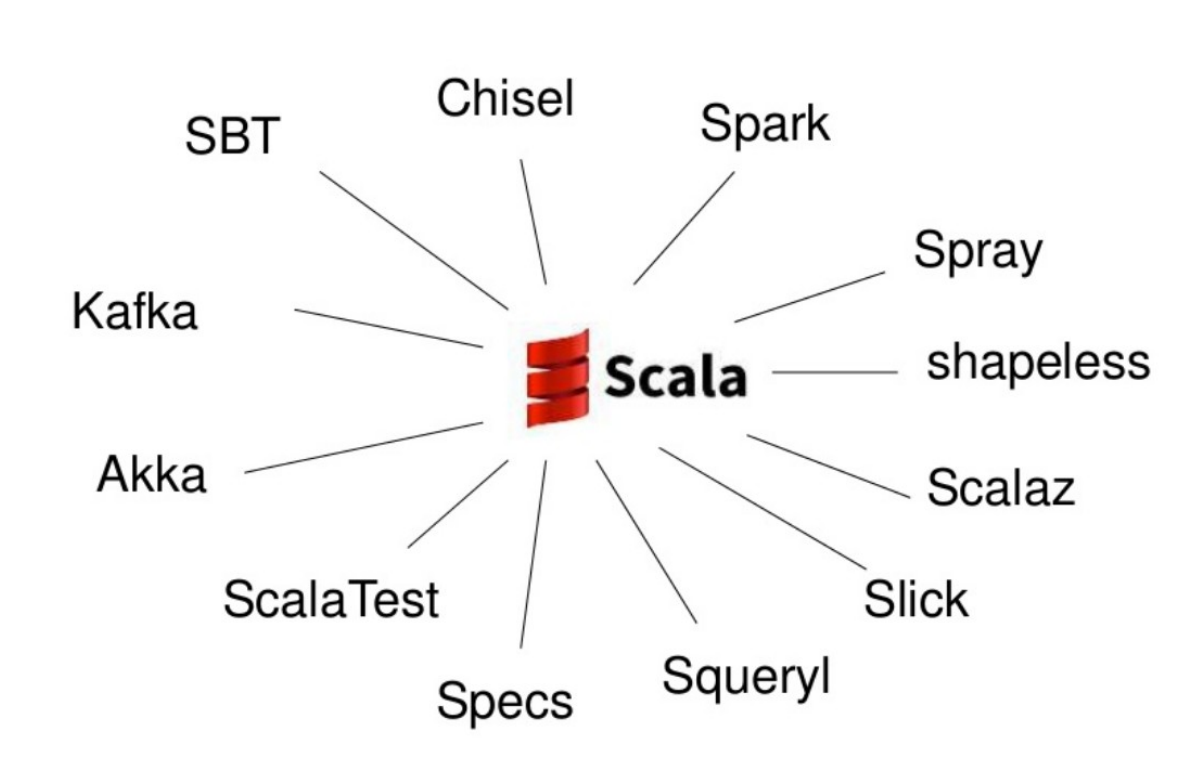
\includegraphics[scale=0.27]{slike/scalaDer}
  \caption{Окружења која користе Скалу}
  \label{fig:scalaDer}
\end{figure}

\subsubsection{Функције вишег реда}
\ac{fvr} су општи концепт који се јавља како у функционалном програмирању тако и математици. Функционални језици третирају функције као „грађане првог реда”, а то значи да:
\begin{itemize}
 \item функција може бити прослеђена као параметар другој функцији
 \item функција може бити резултат друге функције
\end{itemize}

Пример употребе \acs{fvr} за сумирање \cite{courseraHOF}:

\begin{minted}[frame=single,framesep=6pt]{scala}
def sum(f: Int => Int, a: Int, b: Int): Int =
  if a > b then 0
  else f(a) + sum(f, a + 1, b)

def id(x: Int): Int = x
def cube(x: Int): Int = x * x * x
def fact(x: Int): Int = if x == 0 then 1 else x * fact(x - 1)

def sumInts(a: Int, b: Int) = sum(id, a, b)
def sumCubes(a: Int, b: Int) = sum(cube, a, b)
def sumFactorials(a: Int, b: Int) = sum(fact, a, b)
\end{minted}

Овде се може приметити да функција \verb+sum()+ користи функцију \verb+f()+  као параметар, такође има и доњу границу \verb+a+ и горњу границу \verb+b+. Посебно су дефинисане функције \verb+sumInts()+ (сума бројева), \verb+sumCubes()+ (сума кубних вредности) и \verb+sumCubes()+ (сума факторијела бројева) на опсегу од \verb+a+ до \verb+b+. Може се приметити да су једине разлике њихових дефиниција функције која се прослеђује као аргументи \verb+id()+, \verb+cube()+ и \verb+fact()+.
Такође, функције \verb+sumInts()+ (сума бројева) и \verb+sumCubes()+ је могуће дефинисати и употребом \textbf{Анонимних функција}:
\begin{minted}[frame=single,framesep=6pt]{scala}
def sumInts(a: Int, b: Int) = sum(x => x, a, b)
def sumCubes(a: Int, b: Int) = sum(x => x * x * x, a, b)
\end{minted}
Овако се може избећи писање великог броја кратких функција. Функцију \verb+sum()+ је могуће дефинисати и тако да није неопходно прослеђивати \verb+a+ и \verb+b+ при дефинисању функција за различита сумирања.
\begin{minted}[frame=single,framesep=6pt]{scala}
def sum(f: Int => Int): (Int, Int) => Int =
  def sumF(a: Int, b: Int): Int =
    if a > b then 0
    else f(a) + sumF(a + 1, b)
  sumF
// или скраћено
def sum(f: Int => Int)(a: Int, b: Int): Int =
  if a > b then 0 else f(a) + sum(f)(a + 1, b)
// где би сумирање кубова било овако дефинисано
def sumCubes = sum(x => x * x * x)
// или чак ни то није неопходно..
sum (cube) (1, 10)
\end{minted}
Овакав стил дефинисања и примене функција, где се функција са више параметара може представити у виду секвенце функција једног параметра, назива се \textbf{керификација} (currying).

%\newpage

\subsection{Чизел}
Чизел (енг. \textit{Chisel - Constructing Hardware in a Scala Embedded Language}) је језик за опис хардвера заснован на Скали. Чизел наслеђује аспекте објектно-оријентисаног и функционалног програмирања Скале за опис дигиталног хардвера. Коришћење Скале као основе омогућава опис генератора кола. Чизел код којим су описана кола може бити претворен у Верилог за синтезу и симулацију \cite{wiki_chisel}.

Омогућава корисницима да конструишу хардвер управљајући и повезујући Скала објекте да би се направио граф жељеног хардвера. Чизел бекенд потом анализира резултујући граф да би се добио брз,
циклусно-прецизан \CC\phantom{a}симулатор, који одмах потом може да комуницира са Скала тестним окружењем или Верилог синтезом која ће бити процесирана на FPGA (\textit{Field Programmable Arrays}) интегрисаном колу. Чизел дозвољава генератору хардвера да изврши различита израчунавања у Скали над улазним параметрима током израде графа хардвера. Додатно, програмери могу да искористе одлике функционалног програмирања у Скали за опис апстракција хардвера (нпр.\ имплементација ФИР филтера коришћењем \verb+map+ и \verb+reduce+ функција) и Јава стандардних библиотека (нпр.\ претварање бројева са покретним зарезом у или из репрезентације битова која би се користила у тестном окружењу) као начине за поједностављивање свеукупног развоја хардвера и верификације.
% cite
%
% Остали језици, као SystemVerilog нуде неке могућности које нуди и Чизел као ААААААААААА. Међутим, пошто су ови језици фокусирани на опис хардвера, издвајање делова са генераторима у оне које раде само са параметрима и оне које описују жељени хардвер је више изазовно. Конкретно, имплементација решавача ограничења (constraint solver) се не преводи тако добро у друге језике. Овај решавач, у потпуности написан у Скали,
% користи спецификацију акцелератора (величина FFT, радикс, и број извршних јединица) и производи листу инструкција и мапирања меморије статички гарантоване да неће показивати опасности од меморијских колизија или конфликата банака. Затим, Чизел компоненте генератора користе ову листу за писање ROM-ова за превођење инструкција и IO адреса. Имплементација у другим језицима би изискивала одржавање решавача ограничења ван генератора и комуникацију путем текстуалних фајлова; међутим, ово представља изазове ако интерфејси постану десинхронизовани додавањем функционалности генератора. Такође, Чизел гарантује да се сви описани графикони могу анализирати у синтезибилни Верилог, док се сви системски Верилог аспекти не гарантују да су синтезибилни.

Отклањање грешака током дизајна хардвера у Чизелу може бити изазовно. Дизајнери који користе Чизел често пишу сажет програмски код науштрб коректности. Тако, корисник може да погреши у куцању при дефинисању хардвера, а да не добије никакве грешке. Такође, доста грешака које Чизел враћа су веома нејасне, где само пише ``assertion failed''. На пример, декларисање литерала (непроменљиве вредности) уместо порта унутар улазно-излазних декларација је грешка коју би Чизел ухватио. Међутим, порука о грешци која се добија је донекле бескорисна \cite{berkeley_twigg}.

\subsubsection{Генератори кола и условни изрази}
Сви језици за опис хардвера подржавају писање појединачних инстанци. Међутим, писање инстанци је заморно. Верилог омогућава ограничену параметризацију, као број битова и \verb+generate+ израз, али само толико. Пошто није могуће написати генератор у Верилогу, то би значило да треба да напишемо нову инстанцу, што би дуплирало величину програмског кода.
Генератори би требало (у идеалном случају) да их је могуће направити, да су моћни и да омогућавају прецизну контролу над генерисаним дизајном. Провера грешака је неопходна да бисмо били сигурни ли је композиција дозвољена; без тога, отклањање грешака је тешко. Ово тражи да језик генератора разуме семантику дизајна тј.\ да зна шта јесте, а шта није дозвољено. Такође, генератор не би требало да буде преопширан! Желимо да програм генератора сажето изрази више различитих дизајна, без потребе да се посебно повезује у \verb+if+ условима за сваку инстанцу \cite{git_chisel}.

У наставку је приказан једноставан пример \verb+Passthrough+, који има 4-битни улаз \verb+in+ и 4-битни излаз \verb+out+. Модул повезује \verb+in+ и \verb+out+, па \verb+in+ управља \verb+out+-ом.
%\newpage
\begin{minted}[frame=single,framesep=6pt]{scala}
class Passthrough extends Module {
  val io = IO(new Bundle {
    val in = Input(UInt(4.W))
    val out = Output(UInt(4.W))
  })
  io.out := io.in
}
\end{minted}
\verb+Modul+ је уграђена Chisel класа коју сви хардвер модули морају да наследе. Сви улазни и излазни портови се декларишу у посебној \verb+io+ \verb+val+. Мора да се зове \verb+io+, и мора да буде \verb+IO+ објекат или инстанца у форми \verb+IO(_instantiated_bundle_)+.
\begin{minted}[frame=single,framesep=6pt]{scala}
new Bundle {
    val in = Input(...)
    val out = Output(...)
}
\end{minted}

Декларише се нова хардверска структура типа (\verb+Bundle+) која садржи сигнале \verb+in+ и \verb+out+ са одговарајућим смеровима \verb+Input+ и \verb+Output+, редом. \verb+UInt(4.W)+ представља тип сигнала, у овом случају неозначени (unsigned) цео број ширине 4. Улазни порт се повезује са излазним изразом \verb+io.out := io.in+, и тако \verb+io.in+ управља \verb+io.out+.

Након декларисања Чизел модула, користимо Скалу да позовемо Чизел компајлер да преведе Чизел \verb+Passthrough+ у Верилог \verb+Passthrough+. Овај процес се назива обрађивање (elaboration).
\begin{minted}[frame=single,framesep=6pt]{scala}
println(getVerilog(new Passthrough))
\end{minted}

Као било која Скала класа и Чизел модул би могао да прими неке параметре. У наставку је приказан пример генератор модула, где се дефинише нова класа \verb+PassthroughGenerator+ која прима целобројну вредност \verb+width+ која одређује ширине улазног и излазног порта:
\begin{minted}[frame=single,framesep=6pt]{scala}
class PassthroughGenerator(width: Int) extends Module {
  val io = IO(new Bundle {
    val in = Input(UInt(width.W))
    val out = Output(UInt(width.W))
  })
  io.out := io.in
}

println(getVerilog(new PassthroughGenerator(10)))
println(getVerilog(new PassthroughGenerator(20)))
\end{minted}
Може се приметити да Верилог користи различит број битова за улаз/излаз зависно од параметра \verb+width+.
\begin{minted}[frame=single,framesep=6pt]{verilog}
//Elaborating design...
//Done elaborating.
module PassthroughGenerator(
  input        clock,
  input        reset,
  input  [9:0] io_in,
  output [9:0] io_out
);
  assign io_out = io_in; // @[cmd4.sc 6:10]
endmodule

//Elaborating design...
//Done elaborating.
module PassthroughGenerator(
  input         clock,
  input         reset,
  input  [19:0] io_in,
  output [19:0] io_out
);
  assign io_out = io_in; // @[cmd4.sc 6:10]
endmodule
\end{minted}
% \verb++
Пошто су Чизел модули нормалне Скала класе, можемо да искористимо предност конструктора Скала класа да параметризујемо обрађивање дизајна. Још једном, ову параметризацију омогућава Скала, не Чизел. Пошто \verb+PassthroughGenerator+ не описује само један модул, већ описује породицу модула са параметром \verb+width+, овај модул представља један \textbf{генератор}.

Основни условни изрази у Чизелу су \verb+when+, \verb+elsewhen+ и \verb+otherwise+. За разлику од \verb+if+ услова у Скали, овде се не враћају вредности на крају делова кода везаних за \verb+when+. На пример, израз \verb+val result = when(squareIt) { x * x }.otherwise { x }+ неће радити. Начин да се заобиђе ово ограничење је \verb+Wire+ конструкт. \verb+Wire+ се може налазити на десној или на левој страни \verb+:=+ оператора. Следећи пример зависно од вредности улазног селектора рачуна један од три полинома $x^2 - 2x + 1$, $2x^2 + 6x + 3$ или $4x^2 - 10x - 5$:
\begin{minted}[frame=single,framesep=6pt]{scala}
class Polynomial extends Module {
  val io = IO(new Bundle {
    val select = Input(UInt(2.W))
    val x = Input(SInt(32.W))
    val fOfX = Output(SInt(32.W))
  })
  val result = Wire(SInt(32.W))
  val square = Wire(SInt(32.W))
  square := io.x * io.x
  when(io.select === 0.U) {
    result := (square - (2.S * io.x)) + 1.S
  }.elsewhen(io.select === 1.U) {
    result := (2.S * square) + (6.S * io.x) + 3.S
  }.otherwise {
    result := (4.S * square) - (10.S * io.x) - 5.S
  }

  io.fOfX := result
}
\end{minted}

\subsubsection{Регистри}
Основни елемент у Чизелу за чување стања је регистар означен са \verb+Reg+. Он чува своју излазну вредност до следеће растуће ивице тактног циклуса, након које узима вредност са улаза. Чизел има имплицитно дефинисан такт који користи сваки регистар у дизајну, па није потребно дефинисати исти тактни сигнал изнова \cite{git_chisel}.

Следећи програмски код приказује имплементацију модула који узима улаз, повећава му вредност за 1, а потом додељује ову вредност улазу регистра. (Имплицитни такт може бити „прегажен” за дизајн са више тактних сигнала.)
\begin{minted}[frame=single,framesep=6pt]{scala}
class RegisterModule extends Module {
  val io = IO(new Bundle {
    val in  = Input(UInt(12.W))
    val out = Output(UInt(12.W))
  })
  val register = Reg(UInt(12.W))
  register := io.in + 1.U
  io.out := register
}
test(new RegisterModule) { c =>
  for (i <- 0 until 100) {
    c.io.in.poke(i.U)
    c.clock.step(1)
    c.io.out.expect((i + 1).U) } }
println("SUCCESS!!")
\end{minted}

Регистар се креира позивом функције \verb+Reg(tpe)+, где је \verb+tpe+ променљива коja кодира тип регистра који желимо. У овом примеру, \verb+tpe+ је \verb+UInt+ дужине 12 бита. Између позива функције \verb+poke()+ и \verb+expect()+, се налази позив функције \verb+step(1)+. Ово обавештава тестни оквир да „окине” један тактни сигнал, што ће довести до преноса улазних података из регистра на његов излаз. Позив функције step(n)+ ће откуцати тактни сигнал \verb+n+ пута.
Тестери који тестирају комбинаторну логику не позивају \verb+step()+. Ово је зато што позив функције \verb+poke()+ на улазу одмах прослеђује ажуриране вредности кроз комбинаторну логику. Позив функције \verb+step()+ је потребан само за ажурирање елемента стања у секвенцијалној логици.

Блок кода испод ће приказати део Верилог код који је генерисан помоћу \verb+RegisterModule+.
Променљива register се приказује као \verb+reg [11:0]+, као што се и очекивало.
Постоји блок секције \verb+ifdef Randomize+ који иницијализује регистар на неку случајну вредност пре почетка симулације.
Регистар се ажурира на позитивну ивицу такта. Позивом \verb+getVerilog(new RegisterModule)+ добија се 60 линија Верилог програмског кода.
\begin{minted}[frame=single,framesep=6pt]{verilog}
module RegisterModule(
  input         clock,
  input         reset,
  input  [11:0] io_in,
  output [11:0] io_out
);
`ifdef RANDOMIZE_REG_INIT
  reg [31:0] _RAND_0;
`endif // RANDOMIZE_REG_INIT
  reg [11:0] register; // @[cmd2.sc 7:21]
  assign io_out = register; // @[cmd2.sc 9:10]
  always @(posedge clock) begin
    register <= io_in + 12'h1; // @[cmd2.sc 8:21]
  end
  ...
\end{minted}

Претходно дефинисани модул се може скратити коришћењем \verb+RegNext+, па би излаз модула био дефинисан као \verb-io.out := RegNext(io.in + 1.U)-. Верилог код оваквог модула би изгледао готово исто као у претходном примеру.

Регистар у модулу \verb+RegisterModule+ је иницијализован случајним подацима за потребе симулације. Осим ако није другачије наведено, регистри немају вредност ресетовања (или ресет). Начин за креирање регистра који се ресетује на одређену вредност је коришћењем функције \verb+RegInit+. Па би излазна вредност модула била дефинисана као:
\begin{minted}[frame=single,framesep=6pt]{scala}
val register = RegInit(0.U(12.W))
register := io.in + 1.U
io.out := register
\end{minted}
Верилог код се добије из овако дефинисаног модула имао био блок који врши проверу \verb+if(reset)+ где се регистар ресетује на 0. Овај блок се налази унутар блока \verb+always @(posedge clock)+. Регистар се опет иницијализује на насумичну вредност, пре него што се изврши ресет.

Регистри су веома слични жицама (\verb+wire+) у Чизелу по питању контроле тока. Могу им се додељивати вредности употребом \verb+when+, \verb+elsewhen+ и \verb+otherwise+.

\begin{minted}[frame=single,framesep=6pt]{scala}
val max = RegInit(0.U(10.W))
  when (io.in > max) {
    max := io.in
  }
\end{minted}

Операције над регистрима се изводе над његовим излазом, и врсте операција зависе од тога ког је типа регистар. Ако је је регистар типа \verb+UInt+ и дефинисан као \verb+val reg: UInt = Reg(UInt(4.W))+, то значи да су могуће све операције које дозвољава тип \verb+UInt+, као \verb-+-, \verb+-+ \dots

\subsubsection{Типови и оператори}
Потребно је правити разлику између Скала и Чизел типова. На следећем примеру се може видети нпр.\ разлика између \verb+UInt+ из Чизела и \verb+Int+ из Скале. У реду је доделити \verb+a+ вредност \verb+0.U+, а ако би се доделила вредност \verb+0+ дошло би до грешке.
\begin{minted}[frame=single,framesep=6pt]{scala}
val a = Wire(UInt(4.W))
a := 0.U  // legal
a := 0    // illegal
\end{minted}

Чизел тип \verb+Bool+ и Скала тип \verb+Boolean+ се разликују. Код условних израза ово долази до изражаја, па ја у случају услова \verb+when+ могуће користити само \verb+Bool+, а у \verb+if+ је могуће поставити као услов \verb+Boolean+; мешање доводи до грешке.

Такође, није дозвољено комбиновање типова нпр.\ \verb-1.U + 1-. Операције одузимања или множења се изводе на неозначеним бројевима нпр.\ \verb+io.out_add := 1.U * 4.U+.

Чизел има уграђене операторе \verb+Mux+ (мултиплексер) и \verb+Cat+ (надовезивање), где би у наредном примеру \verb+Mux+ вратио \verb+3.U+ уколико је \verb+s+ тачно, а \verb+Cat+ би извршио надовезивање бинарних репрезентација бројева и излаз је 101.
\begin{minted}[frame=single,framesep=6pt]{scala}
io.out_mux := Mux(s, 3.U, 0.U)
io.out_cat := Cat(2.U, 1.U)
\end{minted}


\subsection{Јупитер свеска и Докер}
Током савладавања Чизела кроз приручник (Chisel Bootcamp), наведеном у литератури \cite{git_chisel}, било је потребно користи за његовo покретање платформу Докер (Docker), а сам приручник је приказан у Јупитер свесци (Jupyter notebook). Јупитер свеска омогућава извршавање делова кода и није потребно извршавати целу скрипту сваки пут. Развој имплементације изложене у овом раду је започет у оквиру овог туторијала, али у случају грешке поруке нису биле довољно јасне (или програм није терминирао), па је било неопходно извршавати команде локално кроз \verb+sbt+.

\subsection{Intellij и SBT}
Развој рекурзивне имплементације је рађен у IntelliЈ развојном окружењу, а за компајлирање и тестирање програма је коришћен алат SBT - Scala (Simple) Build Tool, где се команде покрећу у терминалу директоријума пројекта (нпр.\ \verb+sbt+).

\subsection{Quartus Prime Lite}
Синтеза кола имплементираних у Верилогу је рађена у софтверу Quartus Prime Lite компаније Intel, који се користи за дизајнирање програмабилних логичких кола. Поред саме синтезе, коришћене су функционалности софтвера као RTL View који омогућава приказ слике добијеног кола и симулација уз помоћ EDA алата Questa. Коришћене су бесплатне верзије ових алата.

\newpage
\section{Мреже за сортирање}
Сортирање је одувек био фундаментални проблем у рачунарству и детаљно је изучаван. Постоје разни методи сортирања за софтверске и хардверске имплементације. У случају хардверских, постоји компромис између пропусне способности и цене (тј.\ логике и меморије за сортирање $n$ елемената). Два популарна решења су битоник мрежа за сортирање и линеарни сортер. За листу дужине $n$, битоник сортер захтева $\mathcal{O}(n \log^2 n)$ логике и меморије и може да сортира $n$ елемената по циклусу; линеарни сортер захтева $\mathcal{O}(n)$ логике и меморије и сортира $n$ елемената за $n$ циклуса \cite{zuluaga2016}.

Сада ће бити дефинисани неопходни кључни термини за описивање својстава различитих решења.
\begin{definition}[Пропуштање]
Замислимо хардверски дизајн који мора да прими $n$ речи података (и да врати $n$ речи података на излазу). Ако прими (и врати) $w$ речи по тактном циклусу током $n/w$ узастопних циклуса, ово се назива \textit{пропуштање} (\textit{streaming}), где је $w$ пропусна ширина.
\end{definition}
Имплементирањем дизајна са пропусном ширином $w$ мањом од $n$ (број речи који се сортира), цена и улазно-излазна пропусна способност система се смањују.
\begin{definition}[Потпуно пропуштање]
Дизајн који константно може да прима улазни ток података без икаквог времена чекања између два улазна скупа се назива \textit{потпуно пропустан} (\textit{fully streaming}) дизајн.
\end{definition}
Потпуно пропусна мрежа за сортирање пропусне ширине $w$ ће имати пропусну способност $w$ речи по тактном циклусу. Обично се може очекивати да потпуно пропустан дизајн захтева више ресурса од дизајна која није потпуно пропустан, зато што за исто време обрађује више података.

\textit{Мреже за сортирање} паралелно обрађују листу $n$ улазних елемената кроз више нивоа тако да је на последњем нивоу улазна листа сортирана. Током сваког нивоа паралелно се изводе поређења и пермутације. Број нивоа који је потребан да се добије сортирана листа и број поређења по нивоу одређују цену мреже. Број улазних вредности је степен броја два: $n = 2^t$.

Слика \ref{fig:bitonicStages} показује \textit{битоник} (енг. \textit{bitonic}) мрежу за сортирање \cite{bitonicBatcher}. Има осам улазних елемената. Оператор $S_2$ сортира два улаза у растућем редоследу. Мреже за сортирање могу да постигну веома велику пропусност, зато што су потпуно пропусне, где је ширина протока $n$. Обично су повезане тако да се одржи разумна брзина такта и тада је потребно $\mathcal{O}(n \log^2 n)$ флип-флопова за меморију.
\begin{figure}[H]
  \centering
      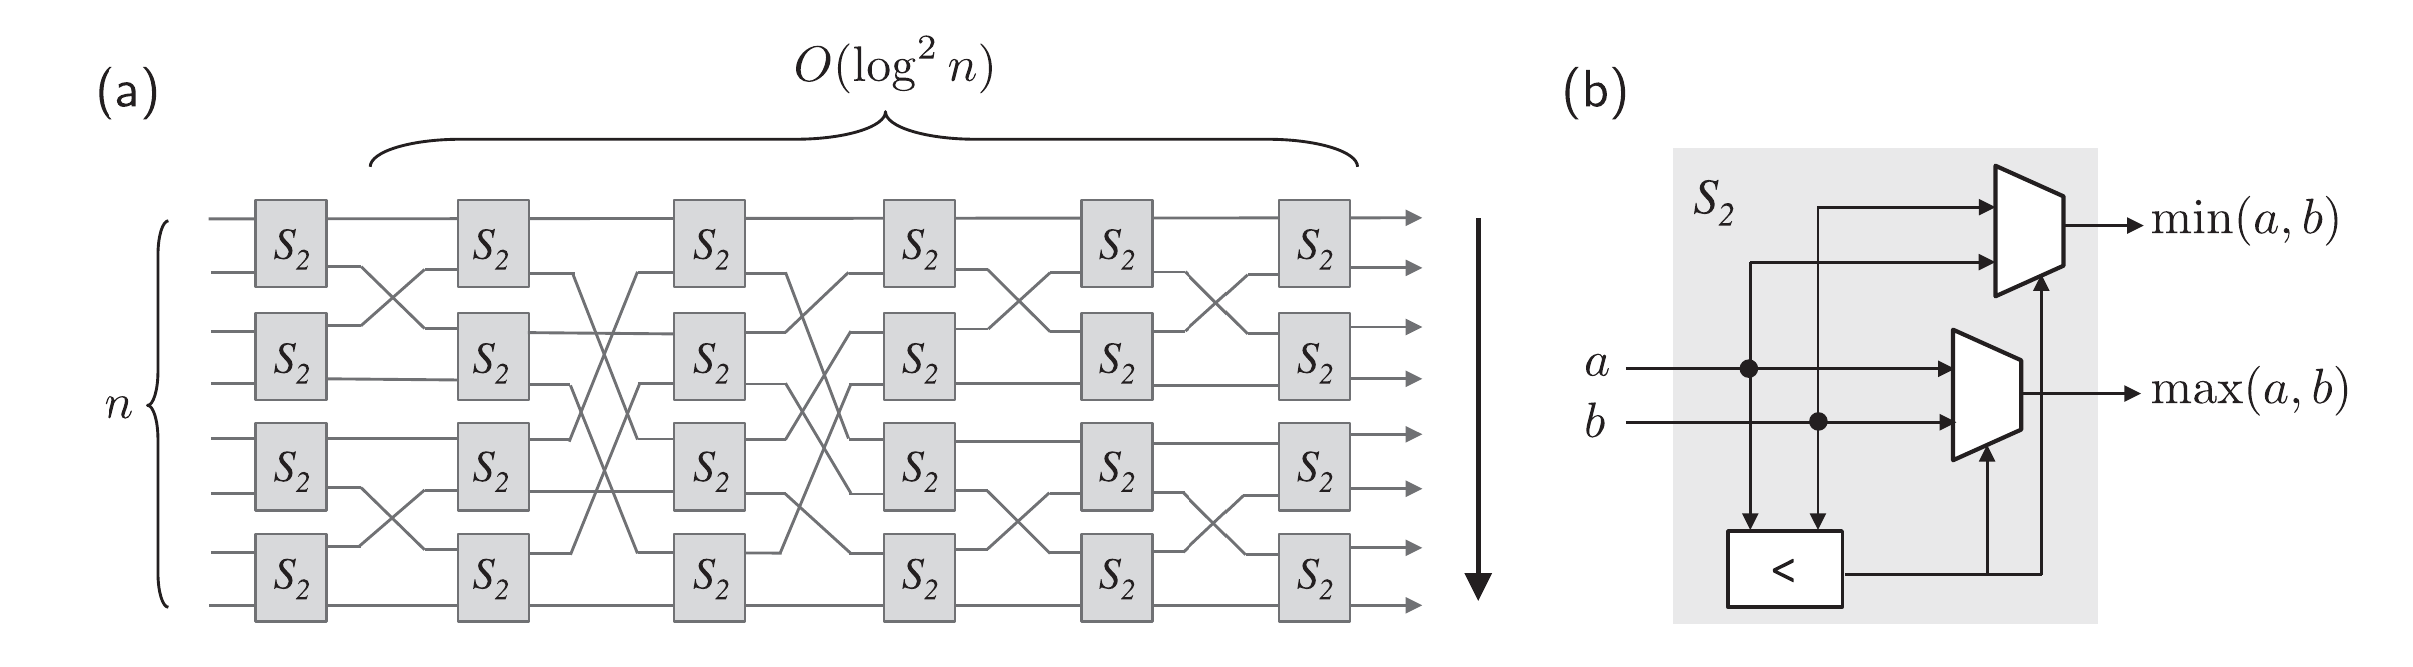
\includegraphics[scale=0.24]{slike/bitonicStages.png}
  \caption{(a) Битоник мрежа за сортирање за улазну величину скупа $n = 8$ \mbox{(b) Двоулазни} сортер $S_2$ је градивна јединица у мрежама за сортирање}
  \label{fig:bitonicStages}
\end{figure}
Као што се може приметити на слици \ref{fig:bitonicStages}, битоник мрежа за сортирање има константну структуру и може се конструисати рекурзивно. Сортира се $n$ елемената у $\log_{2}(n)(\log_{2}(n)+1)/2$ нивоа са $n/2$ паралелних $S_2$ операција, па је потребно $\mathcal{O}(n\log^2 n)$ операција поређења. Кенет Едвард Бечер (Kenneth Edward Batcher) је објавио овај алгоритам 1968.\ године, а такође је развио и \textit{пар-непар} (\textit{odd-even}) мреже за сортирање, које имају мање константну структуру, али захтевају мало мање операција поређења.
Пар-непар и битоник мреже за сортирање су остале најпопуларнија решења због своје једноставности и скоро оптималне цене и перформанси.

\textit{Линеарни сортер} је линеарни низ $n$ чворова који сортирају $n$ вредности, где $n$ није ограничено да мора да буде степен броја два. Сваки чвор се састоји од флип-флопа и оператора поређења. Асимптотско време и логичка цена линеарних сортера је $\mathcal{O}(n)$ и оне су потпуно пропусне са пропусном ширином 1.
%сортирање спајањем ()

\subsection{Битоник сортер}
Низ бројева може да се назове битоник ако се састоји од два монотона низа, једног растућег и другог опадајућег. Такође, низ остаје битоник ако је подељен било где и два дела замењена.

Ако је низ $2n$ бројева $a_1, a_2, \dots, a_{2n}$ битоник и ако направимо два низа од $n$ бројева
\begin{equation}
 min(a_1, a_{n+1}), min(a_2, a_{n+2}), \dots, min(a_n, a_{2n})
 \label{eq:bit1}
\end{equation}
\begin{equation}
 max(a_1, a_{n+1}), max(a_2, a_{n+2}), \dots, max(a_n, a_{2n})
 \label{eq:bit2}
\end{equation}
онда су оба ова низа битоник и ниједан број из (\ref{eq:bit1}) није већи ни од једног броја из низа (\ref{eq:bit2}). Одавде се долази до итеративног правила приказаног на слици \ref{fig:batcherIter}. Битоник сортер за $2n$ бројева може бити конструисан од $n$ елемената за поређење и два битоник сортера за $n$ бројева. Елементи за операцију поређења формирају два низа (\ref{eq:bit1}) и (\ref{eq:bit2}) и пошто су оба битоник сортирају се са два битоник сортера за $n$ бројева. Пошто ниједан број из (\ref{eq:bit1}) није већи ни од једног броја из низа (\ref{eq:bit2}) излаз из једног битоник сортера је доња половина сортираног низа, а излаз другог сортера је горња половина \cite{bitonicBatcher}.

\begin{figure}[H]
  \centering
      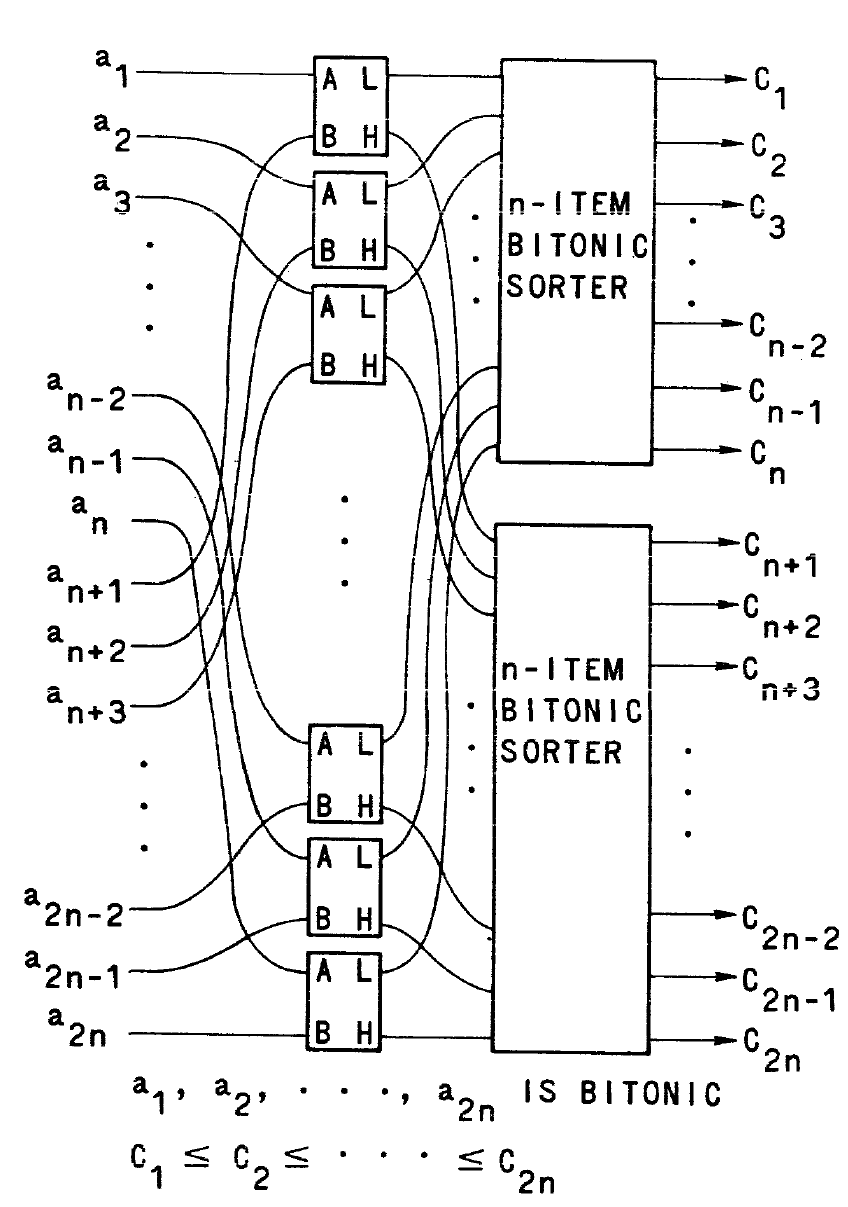
\includegraphics[scale=0.4]{slike/batcherIter}
  \caption{Итеративно правило за битоник сортере}
  \label{fig:batcherIter}
\end{figure}

Битоник сортер за два броја је само један елемент за поређење и коришћењем итеративног правила битоник сортери за $2^p$ бројева могу бити конструисани за било које $p$. Слика \ref{fig:batcher4_8num} приказује приказује сортере за четири и осам бројева. Битоник сортер за $2^p$ бројева захтева $p$ нивоа по $2^{p-1}$ елемената, укупно $p2^{p-1}$. Може да се искористи као мрежа за спајање за било које две листе укупне дужине $2^p$.

\begin{figure}[H]
  \centering
      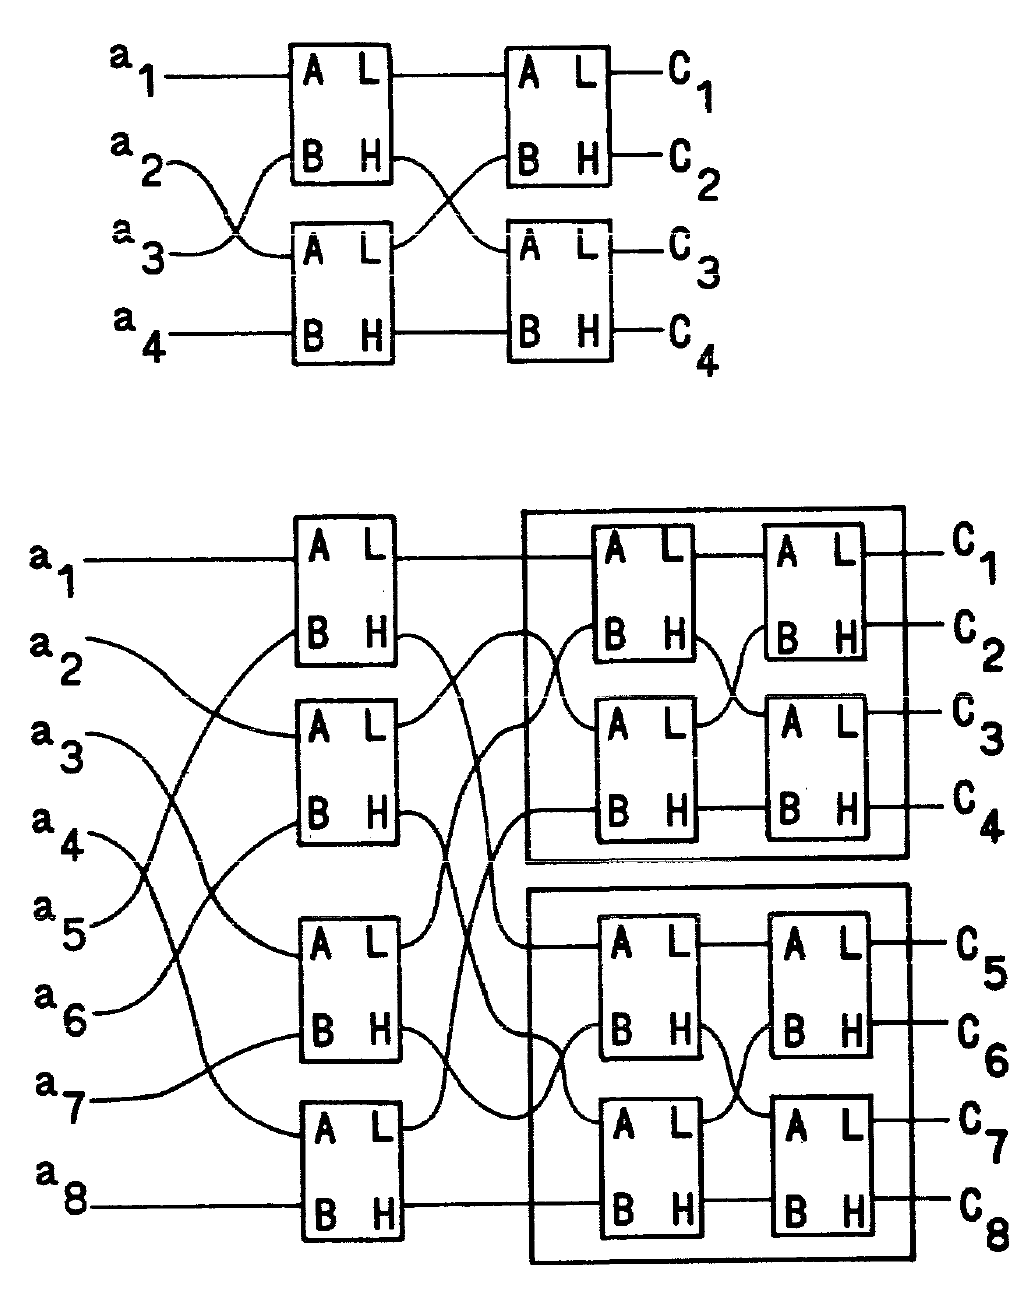
\includegraphics[scale=0.3]{slike/batcher4_8num}
  \caption{Конструкција битоник сортера за четири и осам бројева}
  \label{fig:batcher4_8num}
\end{figure}

Велики битоник сортери могу бити конструисани из више мањих битоник сортера. На слици \ref{fig:batcher16num} је приказан битоник сортер за 16 бројева конструисаног од осам битоник сортера за 4 броја.

\begin{figure}[H]
  \centering
      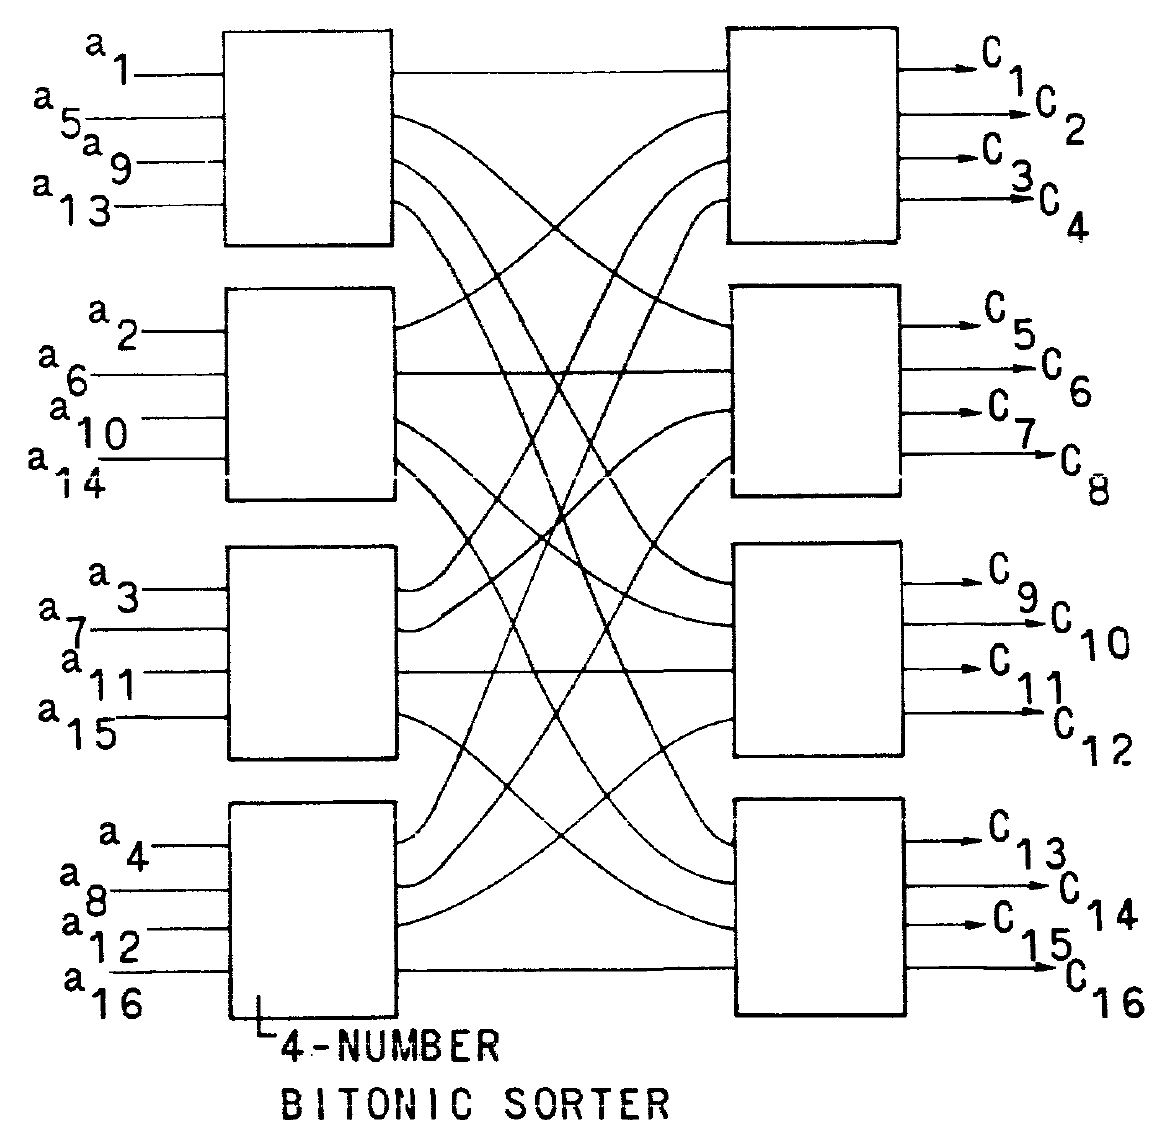
\includegraphics[scale=0.3]{slike/batcher16num}
  \caption{Битоник сортер за 16 бројева конструисаног од осам битоник сортера за 4 броја}
  \label{fig:batcher16num}
\end{figure}

Следећа слика боље приказује како ради алгоритам. 16 бројева се налази на улазу на левој страни и прелазе преко 16 хоризонталних жица до излаза на десној страни. Мрежа сортира елементе, тако да се највећи налази на дну.

Стрелице представљају операције поређења и показују ка већем броју. Уоквирени правоугаоници у боји немају утицај на рад алгоритма, само олакшавају разумевање.
\begin{figure}[H]
  \centering
      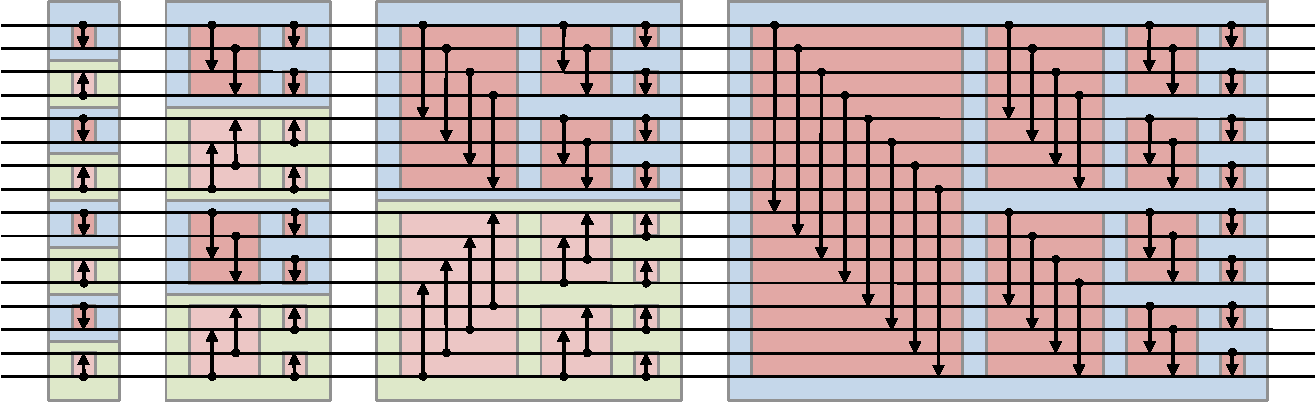
\includegraphics[scale=0.7]{slike/BitonicSort1.pdf}
  \caption{Приказ рада битоник алгоритма са 16 бројева на улазу}
  \label{fig:bitonicSortWiki}
\end{figure}
Ако се осматрају црвени правоугаоници, може се приметити да се сваки улаз из горње половине пореди са одговарајућим улазом који се налази у доњој половини правоугаоника, где су стрелице усмерене надоле ако су у питању тамноцрвени правоугаоници или нагоре код светлоцрвених.
%
Ако бројеви на улазу формирају битоник низ, онда ће се на излазу наћи два битоник низа. Горња и доња половина излаза ће бити битоник, где ће сваки број горње половине бити мањи (или једнак) од сваког из доње (у тамноцрвеним) или обрнуто (у светлоцрвеним) \cite{wiki_bitonic}.
%
\begin{figure}[H]
  \centering
      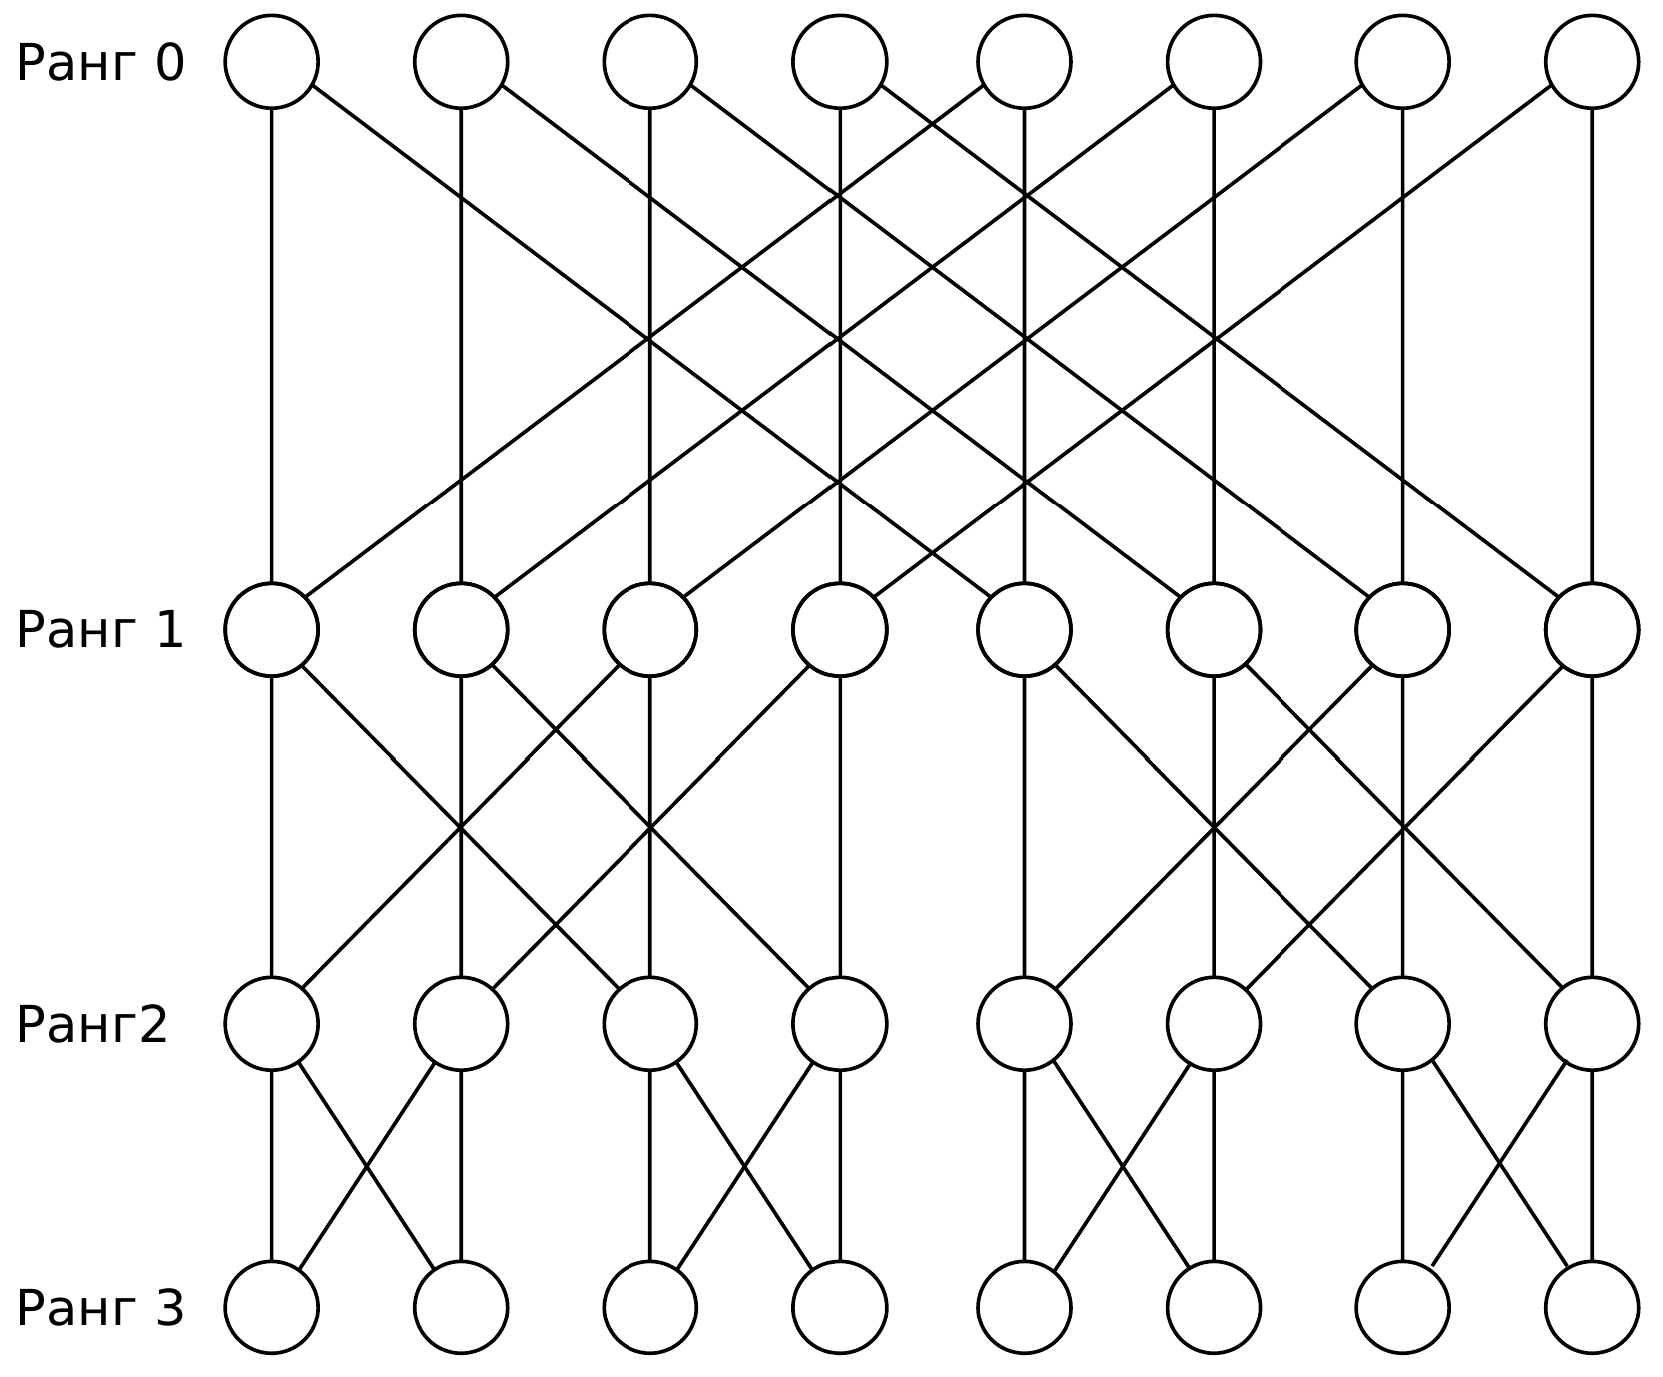
\includegraphics[scale=0.16]{slike/leptir}
  \caption{Топологија лептира}
  \label{fig:leptir}
\end{figure}
Црвени правоугаоници формирају плаве и зелене. Црвени примају цео улазни низ, потом половину резултата, потом половину тих резултата итд. Све стрелице показују надоле (плави) ил нагоре (зелени). Ова структура је позната као лептир (buterfly) мрежа. Топологија лептира је приказана на слици \ref{fig:leptir}. Ако се на улазу у овакав правоугаоник нађе битнок низ, онда ће излаз бити сортиран у растућем поретку у слчају плавих правоугаоника или опадајућем код зелених. Када се број налази на улазу у зелени или плави правоугаоник, онда ће први црвени да га сортира у праву половину листе. Потом пролази кроз мањи црвени правоугаоник који га сортира у праву четвртину листе унутар те половине итд. Излаз из зеленог или плавог правоугаоника је потпуно сортиран.

Коришћењем плавих и зелених правоугаоника се може направити цела мрежа. Излаз из сваког зеленог и плавог правоугаоника је сортиран низ, па ће излаз сваког пара суседних низова бити битоник, зато што је горњи плави, а доњи зелени. Свака колона плавих и зелених правоугаоника узима $N$ сортираних низова и спаја их у паровове тако да се добије $N/2$ битоник низова, који се потом сортирају унутар правоугаоника те колоне да се добије $N/2$ низова. Овај процес почиње од сортиране листе која садржи један елемент и наставља се кроз све колоне док се у последњој колони не споје у једну сортирану листу. Пошто је последњи ниво плави, коначна листа ће имати највећи елемент на дну. \cite{wiki_bitonic}.

\subsection{Други сортери}
Стоун \cite{stone} је развио битоник мреже за сортирање са константном геометријом (1971). Ово значи да су две суседне фазе поређења од n/2 паралелних поређења увек повезане истом пермутацијом - такозваним савршеним мешањем. Тако се мрежа може пресавити (fold) тако да се користи само једна фаза поређења и мешања, кроз коју се подаци крећу $\mathcal{O}(\log_{2} n)$ пута. Смер поређења се мења током фаза, што захтева мали додатни простор за контролну логику.

Слични напори да се пресавије или регулише битоник мреже за сортирање предложени су касније. Дауд и други \cite{dowd} предлажу периодичну балансирану мрежу за сортирајућу која постиже различиту грануларност поновне употребе са блоком од $\log n$ фаза који се може користити $\log n$ пута. С друге стране, Лајер и други \cite{layer07} предлажу битоник мрежу за сортирање коју чини $\log_{2} n$ фаза које више пута круже са подацима унутар сваке фазе (1989).

Ограничење већине паралелних архитектура за сортирање са фиксним рачунарским током, као што су мреже за сортирање, је да морају увек сортирати улазне сетове исте величине. Решење за ово је адекватно додавање улазног сета тако да се елементи који се сортирају налазе на врху излазне листе. Лајер и Пфлајдерер \cite{layer04} предложили су архитектуру која може подржавати различите величине улаза, до фиксног максимума (2004). Прилагодљива логика се користи за промену неопходних мешања у зависности од ширине улаза. Други приступ, представљен у раду Занг и Женг \cite{zang}, користи серијску мрежу за сортирање са фиксном величином улазног сета \verb+m+ и скупом од \verb+m+ редова, сваки од којих може садржавати \verb+n/m+ елемената (2000). Контролнa логикa је потребна да адекватно подржи мрежу за сортирање.
Предложене су и мрежу за сортирање са бољом асимптотском ценом. Посебно, Ајтаи и други \cite{aitan} представљају АКС сортирајућу мрежу, која има оптималну асимптотску цену од $\mathcal{O}(n\log n)$ (1983). На жалост, ови резултати имају чисто теоријску вредност, јер велика скривена константа чини ове мреже неупотрбљивим у пракси.

Друга мрежа за сортирање која је популарна због своје високе регуларности и једноставности је пар-непар мрежа за сортирање са премештањем (transposition) \cite{knuth}, која међутим захтева $\mathcal{O}(n)$ фаза и $\mathcal{O}(n^2)$ операција поређења (1968). Као и у случају Стоун-а \cite{stone}, она се може пресавити тако да се користи само једна фаза $\mathcal{O}(n)$ пута.

На крају, пар-непар мрежа за сортирање и битоник мреже за сортирање остају најпопуларнија решења због своје једноставности и близине оптималној цени и перформансама.

\newpage

\section{Постојећа решења}
%Поглавље \ref{sec:a_prilog}

Сада ће бити приказане две имплементације које су биле основа за израду оне која је приказана у овом раду.

\subsection{Итеративна имплементација битоник сортера у Чизелу}
Као основа за израду рекурзивног решења изложеног у овом раду је послужила је итеративна имплементација наведена у литератури \cite{git_freeChipsBitonic}.
Програмски код дефинише хардверски модул за извршавање битоник сортирања на броју елемената који је степен броја 2 користећи \verb+Swapper+ модуле за поређење елемената. Дати примери показују како користити битоник сортер модул за конкретне типове података и величине. Сада следи објашњење програмског кода:

\begin{enumerate}
\item Увозе се Чизел библиотеке и дефинише се пакет за битоник сортирање

\item Класа \verb+Swapper+ дефинише хардверски модул за замену два улазна елемента на основу функције поређења. Овај модул има два улаза (\verb+a0+ и \verb+a1+) и два излаза (\verb+z0+ и \verb+z1+).
\begin{minted}[frame=single,framesep=6pt]{scala}
  when(lt(io.a1, io.a0)) {
    io.z0 := io.a1
    io.z1 := io.a0
  }.otherwise {
    io.z0 := io.a0
    io.z1 := io.a1
  } }
\end{minted}


\item Креира се објекат \verb+BitonicSorter+, који је фабрика за креирање битоник сортер хардверских модула. Он прима \verb+IndexedSeq+ (Indexed Sequence) која садржи опционе улазне елеменате \verb+a+ и функцију \verb+factory()+ за креирање \verb+Swapper+ модула. Функција проверава да ли је број елемената за сортирање степен броја 2 и затим врши сортирање елемената користећи битоник алгоритам за сортирање.
\begin{minted}[frame=single,framesep=6pt]{scala}
def insertSorter(a: IndexedSeq[Option[T]], lo: Int, hi: Int):
  IndexedSeq[Option[T]] = { (a(lo), a(hi)) match {
    case (_, None)        => a
    case (None, Some(aH)) => a.updated(lo, Some(aH))
                                .updated(hi, None)
    case (Some(aL), Some(aH)) =>
      val m = Module(factory())
      m.io.a0 := aL
      m.io.a1 := aH
      a.updated(lo, Some(m.io.z0))
        .updated(hi, Some(m.io.z1)) } }
\end{minted}
\begin{itemize}
\item \verb+insertSorter+ је помоћна функција која врши сортирање уметањем у опсегу елемената у a задатим са \verb+lo+ и \verb+hi+. Она врши замену елемената користећи \verb+Swapper+ модуле на основу функције поређења \verb+lt+.

\item Главна логика сортирања се извршава у угњежденој петљи, где \verb+i+ представља битну позицију која
се разматра, \verb+j+ варира од \verb+i+ до \verb+0+, и \verb+k0+ и \verb+k1+ итерирају кроз елементе који требају да се пореде.

\item Унутар петље се проверава да ли је потребна замена елемената користећи \verb+Swapper+ модуле на основу битних позиција и функције поређења.

\item Резултат је сортирана \verb+IndexedSeq+ опционих елемената.
\end{itemize}

\begin{minted}[frame=single,framesep=6pt]{scala}
(for {
      i <- 0 until log2Up(a.length)
      j <- i to 0 by -1
      k0 <- a.indices by (2 << j)
      k1 <- 0 until 1 << j
    } yield {
      val lo = k0 + k1
      val hi = lo + (1 << j)
      if ((lo >> (i + 1)) % 2 == 0) (lo, hi) else (hi, lo)
    }).foldLeft(a) { case (s, (l, h)) => insertSorter(s, l, h) }
\end{minted}


\item Класа \verb+SorterModuleIfc+ дефинише интерфејс за битоник сортер модул. Прима број елемената \verb+n+ и прототип \verb+proto+ за елементе.

\item Дефинише се класа \verb+BitonicSorterModule+ која проширује \verb+SorterModuleIfc+. Ова класа представља битоник сортер модул и прима број елемената \verb+n+, прототип \verb+proto+, и функцију поређења \verb+lt+.

\begin{itemize}
\item Креира се \verb+IndexedSeq+ опционих елемената \verb+a+, иницијализујући га улазним елементима \verb+io.a+. Величина \verb+a+ је постављена на следећи степен броја 2 који је већи или једнак \verb+io.a.length+.

\item Сортирају се елементи \verb+a+ користећи фабрику \verb+BitonicSorter+, наводећи прототип и функцију поређења. Резултат је сортиран \verb+IndexedSeq+ опционих елемената.

\begin{minted}[frame=single,framesep=6pt]{scala}
class BitonicSorterModule[T <: Data](n: Int, proto: T,
      lt: (T, T) => Bool) extends SorterModuleIfc(n, proto) {
private val a = IndexedSeq.tabulate(1 << log2Up(io.a.length))
                  { i => if (i < n) Some(io.a(i)) else None }
io.z := VecInit(BitonicSorter(a, () =>
    new Swapper(proto.cloneType, lt)).slice(0, n).map(_.get))
}
\end{minted}

\item Сортирани елементи се додељују излазу \verb+io.z+.
\end{itemize}


\item Програмски код садржи примере позива кода за генерисање за битоник сортер модула. Дата су два примера за сортирање 64 и 384 елемената 8-битних неозначених целих бројева (\verb+UInt8+) користећи \verb+BitonicSorterModule+.
\newpage
Ови примери генеришу SystemVerilog излаз користећи \verb+ChiselStage+ из Чизела и прослеђују тип и функцију поређења као аргументе.
\begin{minted}[frame=single,framesep=6pt]{scala}
object BitonicSorterUInt8_64Driver extends App {(new ChiselStage)
          .emitSystemVerilog(new BitonicSorterModule(64, UInt(8.W),
                                (x: UInt, y: UInt) => x < y), args)
}
\end{minted}

\end{enumerate}

\subsubsection{Анализа рада итеративне имплементације}
Као што је претходно назначено, главна логика сортирања извршава се у угњежденој петљи, која је изнад приказана.
\begin{table}[H]
\centering
 \begin{tabular}{| c c | c c | c c | c c | c c | c c |}
  \hline
  l & h & l & h & l & h & l & h & l & h & l & h \\
  \hline
  0 & 1 & 0 & 2 & 0 & 1 & 0 & 4 & 0 & 2 & 0 & 1 \\
  3 & 2 & 1 & 3 & 2 & 3 & 1 & 5 & 1 & 3 & 2 & 3 \\
  4 & 5 & 6 & 4 & 5 & 4 & 2 & 6 & 4 & 6 & 4 & 5 \\
  7 & 6 & 7 & 5 & 7 & 6 & 3 & 7 & 5 & 7 & 6 & 7 \\
  \hline
 \end{tabular}
 \caption{Парови индекса бројева који се упоређују}
 \label{tab:index}
\end{table}
Ако бисмо посматрали пример да на улазу имамо низ од осам бројева, и ако бисмо генерисали парове индекса бројева унутар тог низа које је потребно поредити у сваком нивоу (табела \ref{tab:index}), битоник мрежа за сортирање би изгледала као на слици \ref{fig:bitonicIter}.

\begin{figure}[H]
  \centering
      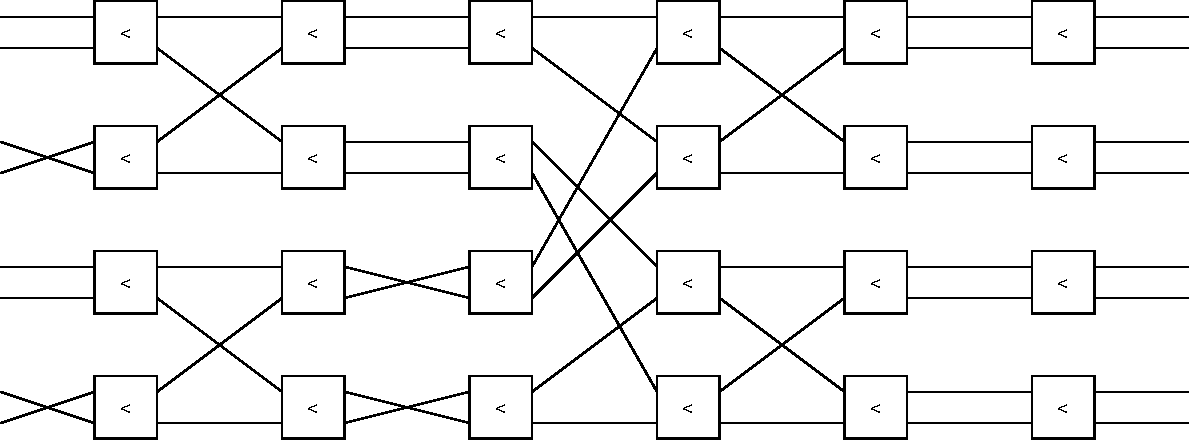
\includegraphics[scale=0.7]{slike/bitonicIter.pdf}
  \caption{Битоник мрежа за сортирање - итеративна имплементација}
  \label{fig:bitonicIter}
\end{figure}

Занимљиво је приметити да је ова мрежа другачија од оне приказане на \mbox{слици \ref{fig:bitonicStages}}. Има исти број нивоа паралелног извршавања операција поређења, али се везе између неких нивоа разликују.

\newpage
На слици \ref{fig:visualizeIter} је приказана визуализација кола извршавањем команде \verb+visualize(()+ => \verb+new BitonicSorterModule(8, UInt(8.W), ...))+

\begin{figure}[H]
  \centering
      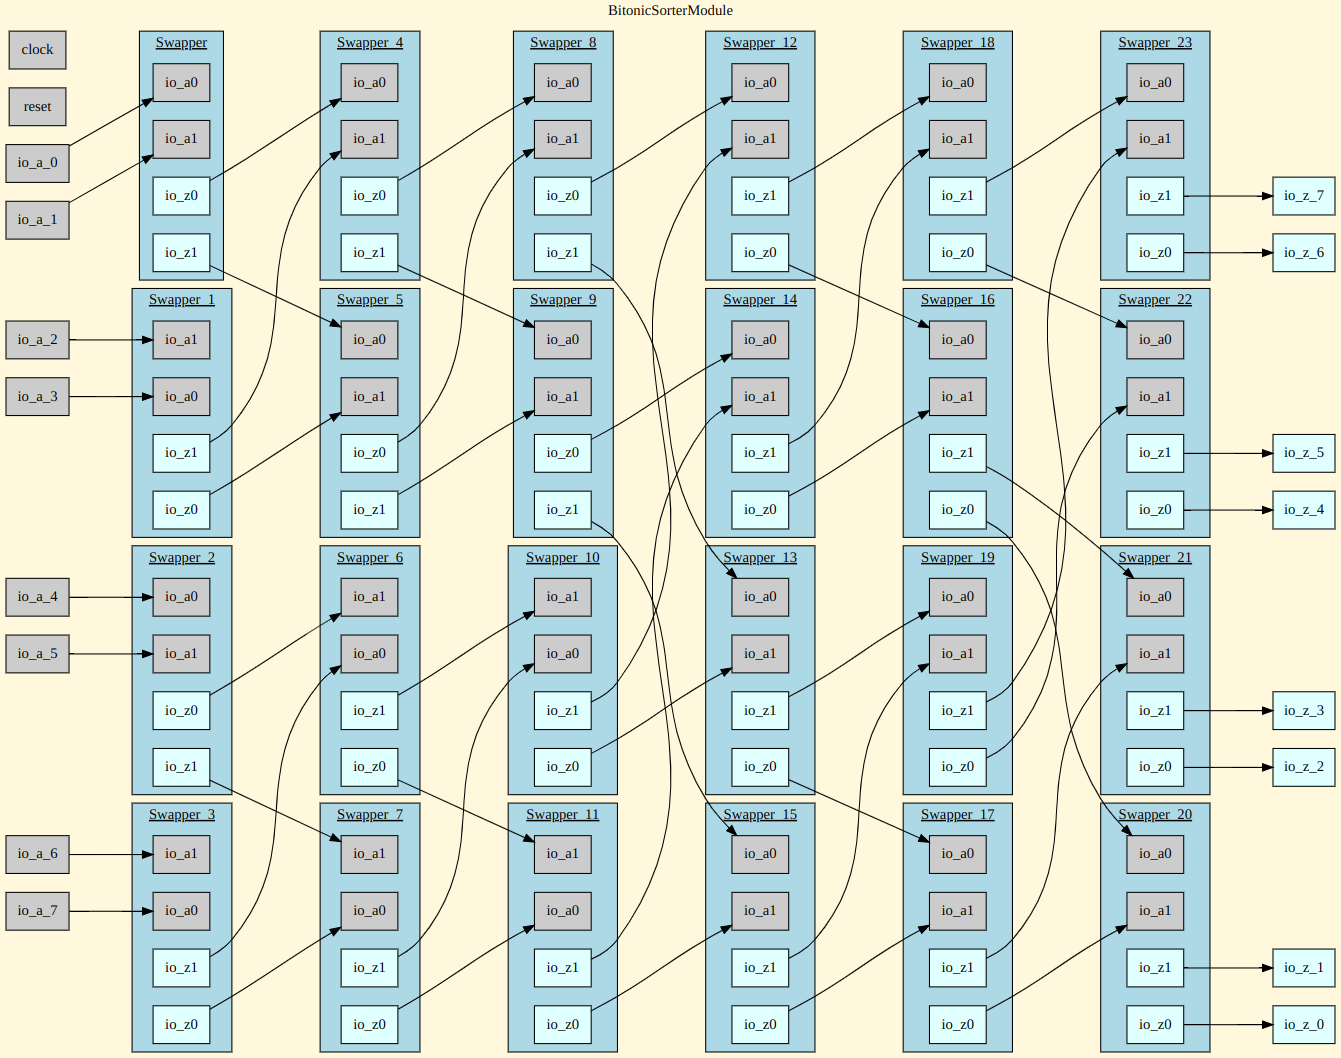
\includegraphics[scale=0.3]{slike/visualizeIter}
  \caption{Визуализација итеративне имплементације}
  \label{fig:visualizeIter}
\end{figure}

Може се приметити да су парови који се пореде исти као у табели \ref{tab:index}.

\subsubsection{Карактеристике генерисаног кола}
Позивом \verb+getVerilog(new BitonicSorterModule(...)+ је добијен Верилог програмски код ове имплементације. Синтеза и симулација рада битоник сортера је урађена у софтверу Quartus Prime Lite, а FPGA уређај коришћен за синтезу је Cyclone V 5CGXFC9E7F35C8.

\begin{table}[H]
\centering
 \begin{tabular}{| c | c | c c |}
  \hline
  Број ел. & Ширина & LUT & Pin \\
  \hline
  8 & 8  & 347 & 130 \\
  8 & 16 & 673 & 258 \\
  8 & 32 & 1669 & 514 \\
  \hline
  16 & 8 & 929 & 258 \\
  16 & 16 & 2154 & 514 \\
  \hline
 \end{tabular}
 \caption{Простор који синтеза заузима за различите величине улаза}
 \label{tab:cipSintezaIter}
\end{table}

Извршена је синтеза за ону величину улаза и излаза колико овај модел има пинова да подржи (616). Табела \ref{tab:cipSintezaIter} приказује колико простора синтеза кода заузима простора на чипу, за различите величине улаза (и излаза). За различит број елемената на улазу и ширину података приказане су у колонама: LUT се односи на број искоришћених Look-Up табела и Pin представља искоришћен број пинова потребних за У/И.

\newpage
Слика \ref{fig:RTL_Iter} приказује генерисано коло за сортирање 16 8-битних елемената на улазу. Moже се приметити да коло значајно расте са порастом броја елемената за сортирање.

\begin{figure}[H]
  \centering
      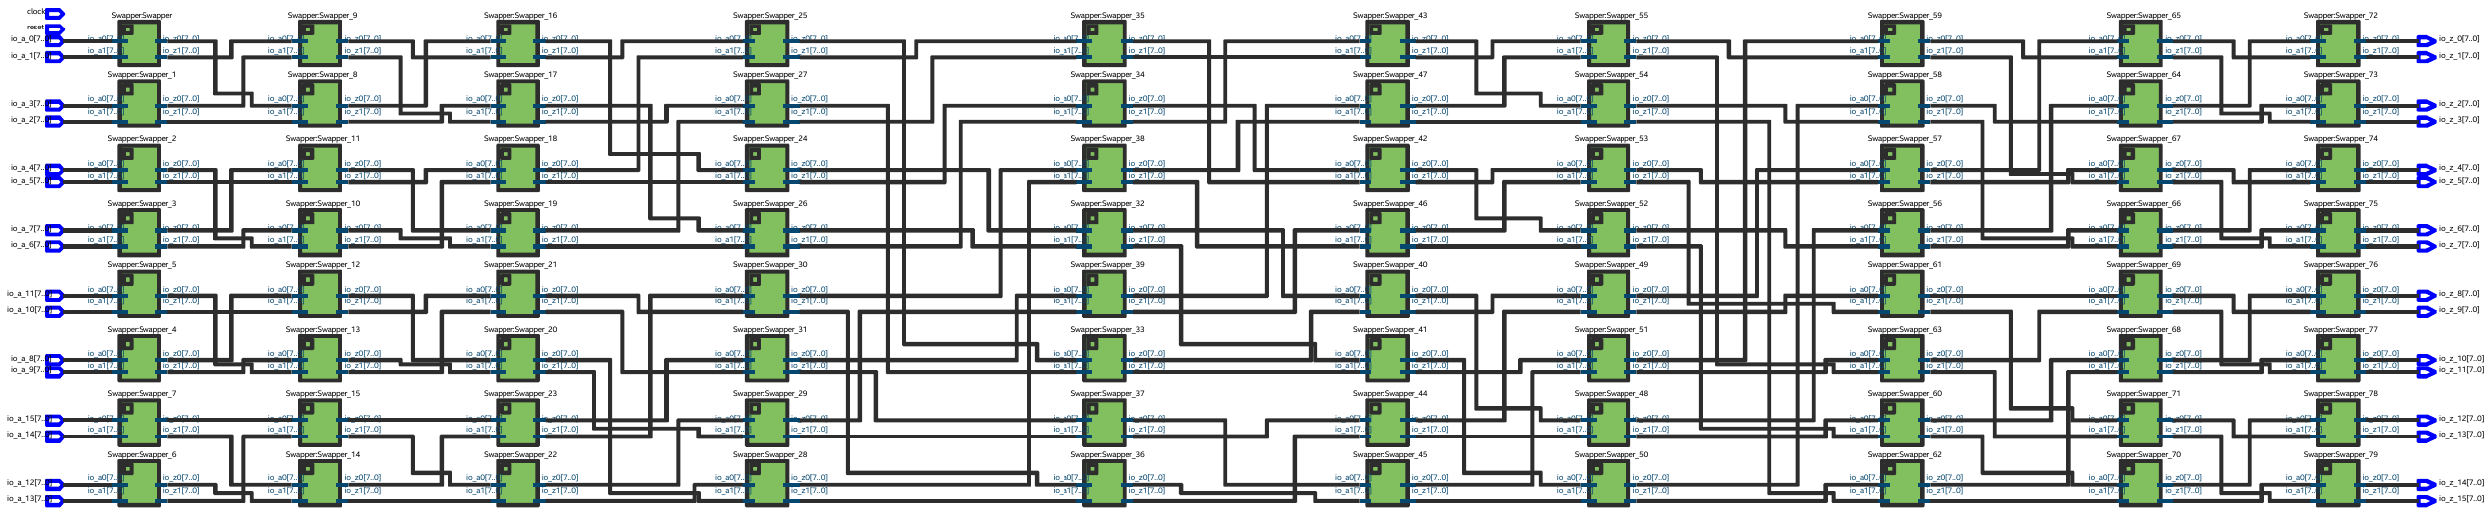
\includegraphics[scale=0.24]{slike/RTL_Iter_16_8.png}
  \caption{Слика добијеног кола за сортирање 16 елемената}
  \label{fig:RTL_Iter}
\end{figure}

Следећа слика приказује један \verb+Swapper+ модул.

\begin{figure}[H]
  \centering
      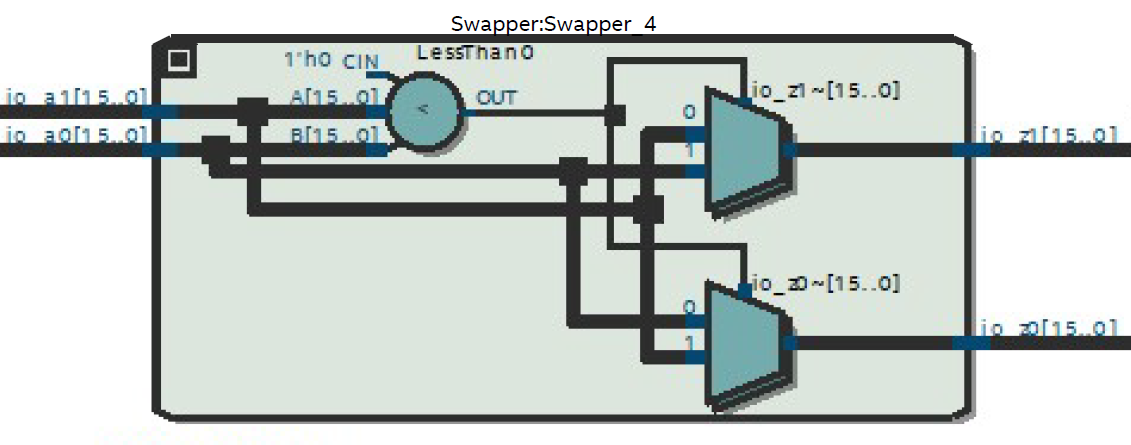
\includegraphics[scale=0.5]{slike/swapper.png}
  \caption{Слика добијеног кола за сортирање 16 елемената}
  \label{fig:swapper}
\end{figure}

\newpage
\subsection{Рекурзивна имплементација у Пајтону}

Логика рекурзивног решења у Чизелу изложеног у овом раду се базира на имплементацији у Пајтону, наведеној у литератури \cite{geeks}.

% Програм функционише само када је величина улазних података степен броја 2. Параметар \verb+dir+ указује смер сортирања, растући или опадајући. Ако услов \verb+a[i] > a[j]+ одговара изабраном смеру, онда се вредности \verb+a[i]+ и \verb+a[j]+ замењују.
%
% Функција \verb+bitonicMerge+ рекурзивно сортира битоник низ у растућем редоследу (ако је \verb+dir = 1+) или у опадајућем редоследу (ако је \verb+dir = 0+). Низ који се сортира почиње на индексу \verb+low+, а \verb+cnt+ је број елемената који треба сортирати.
%
% Ова функција прво производи битонички низ рекурзивним сортирањем његових две половине у супротним редоследима, а затим позива функцију "bitonicMerge" да их уједини у исти редослед.
%
% Позива се функција "bitonicSort" која сортира целокупни низ дужине "N" у РАСТУЋЕМ редоследу.
Сада следи објашњење програмског кода:

\begin{enumerate}
\item \verb+compAndSwap(a, i, j, dire)+ функција служи за упоређивање и замену два елемента у низу a на позицијама \verb+i+ и \verb+j+ у зависности од смера сортирања (уколико је \verb+dire+ једнак 1, онда сортира у растућем редоследу, а уколико је 0, онда сортира у опадајућем редоследу).
\begin{minted}[frame=single,framesep=6pt]{python}
def compAndSwap(a, i, j, dire):
  if (dire==1 and a[i] > a[j]) or (dire==0 and a[i] < a[j]):
      a[i],a[j] = a[j],a[i]
\end{minted}


\item \verb+bitonicMerge(a, low, cnt, dire)+ функција рекурзивно сортира битонички низ у растућем или опадајућем редоследу, у зависности од вредности параметра \verb+dire+. Низ се сортира почевши од позиције \verb+low+, а параметар \verb+cnt+ представља број елемената који се сортирају.
\begin{minted}[frame=single,framesep=6pt]{python}
def bitonicMerge(a, low, cnt, dire):
  if cnt > 1:
    k = cnt//2
    for i in range(low , low+k):
        compAndSwap(a, i, i+k, dire)
    bitonicMerge(a, low, k, dire)
    bitonicMerge(a, low+k, k, dire)
\end{minted}
\item \verb+bitonicSort(a, low, cnt, dire)+ функција прво производи битонички низ рекурзивним сортирањем његових две половине у супротним редоследима, а затим позива функцију \verb+bitonicMerge+ да их уједини у исти редослед.
\begin{minted}[frame=single,framesep=6pt]{python}
def bitonicSort(a, low, cnt,dire):
  if cnt > 1:
    k = cnt//2
    bitonicSort(a, low, k, 1)
    bitonicSort(a, low+k, k, 0)
    bitonicMerge(a, low, cnt, dire)
\end{minted}


\item Из функције \verb+sort(a, N, up)+ се позива сортирање целокупног низа \verb+a+ дужине \verb+N+ у растућем или опадајућем редоследу, у зависности од вредности параметра \verb+up+.

\item Главни део програма почиње креирањем низа \verb+a+ који треба сортирати и подешава величину низа \verb+n+ и смер сортирања \verb+up+. Затим се позива функција \verb+sort(a, n, up)+ да изврши сортирање низа, и на крају се исписује сортиран низ.

\end{enumerate}

\newpage
\subsection{Имплементација битоник сортер у Верилогу}

У овом поглављу ће бити описана имплементација битоник сортера у Верилогу, наведена у литератури \cite{git_verilog}. Описан је програмски код решења и наведене су карактеристике добијеног кола.

Пројекат се састоји од 4 модула \verb+bitonic_node+, \verb+bitonic_comp+, \verb+bitonic_block+ и \verb+bitonic_sort+, где је \verb+bitonic_sort+ на највишем нивоу:
\begin{enumerate}
 \item Модул \verb+bitonic_node+:
 \begin{itemize}
  \item Представља основну јединицу битоник мреже за сортирање.
  \item Користи се за поређење и размену две вредности.
  \item Параметри:
  \begin{itemize}
   \item \verb+DATA_WIDTH+: Представља ширину података тј.\ број битова бинарне репрезентације једног елемента.
   \item \verb+ORDER+: Редослед овог чвора у битоник мрежи.
   \item \verb+POLARITY+: Одређује редослед (улазан или силазан).
   \item \verb+SIGNED+: Одређује да ли су бројеви означени или неозначени.
  \end{itemize}
  \item Улази:
  \begin{itemize}
   \item \verb+clk+: Сигнал такта.
   \item \verb+data_in+: Улазни подаци овог чвора.
  \end{itemize}
  \item Излази:
  \begin{itemize}
   \item \verb+data_out+: Излазни подаци из овог чвора.
  \end{itemize}
  \item Унутар овог модула има више инстанци компоненте \verb+bitonic_comp+ које извршавају стварно поређење и замену.
  \item Користи \verb+generative+ петље да креира и повеже ове инстанце на основу наведених параметара.
  \item Основни циљ модула је да усмери улазне податке кроз битоник мрежу за сортирање и произведе сортиране излазе.
 \end{itemize}

 \item Модул \verb+bitonic_comp+:
 \begin{itemize}
  \item Овај представља компаратор и логику размене за две вредности података.
  \item Параметри:
  \begin{itemize}
   \item \verb+DATA_WIDTH+: Представља ширину података
   \item \verb+POLARITY+: Одређује редослед (улазан или силазан).
   \item \verb+SIGNED+: Одређује да ли су бројеви означени или неозначени.
  \end{itemize}
  \item Улази:
  \begin{itemize}
   \item \verb+CLK+: Сигнал такта.
   \item \verb+A+: Прва улазна вредност.
   \item \verb+B+: Друга улазна вредност.
  \end{itemize}
  \item Излази:
  \begin{itemize}
   \item \verb+H+: Виша од две улазне вредности.
   \item \verb+L+: Нижа од две улазне вредности.
   \item \verb+O+: Излаз који означава да ли је \verb+A+ мање од \verb+B+.
  \end{itemize}
  \item Овај модул пореди улазне вредности \verb+A+ и \verb+B+ и одређује која је виша \verb+H+ и која је нижа \verb+L+.
  \item Такође, производи излаз \verb+O+ који указује да ли је \verb+A+ мање од \verb+B+.
  \item Поларитет компаратора (узлазан или силазан) контролише се параметром \verb+POLARITY+.
  \item Модул користи регистре за чување резултата и ажурира их на сваком такту.
 \end{itemize}

 \item Модул \verb+bitonic_block+:
 \begin{itemize}
  \item Представља степен (ниво) у битоник мрежи за сортирање
  \item Параметри:
  \begin{itemize}
   \item \verb+DATA_WIDTH+: Представља ширину података.
   \item \verb+ORDER+: Редослед овог степена у битоник мрежи.
   \item \verb+POLARITY+: Одређује редослед (улазан или силазан) степена.
   \item \verb+SIGNED+: Одређује да ли су бројеви означени или неозначени.
  \end{itemize}
  \item Улази:
  \begin{itemize}
   \item \verb+clk+: Сигнал такта.
   \item \verb+data_in+: Улазни подаци за овај степен.
  \end{itemize}
  \item Излази:
  \begin{itemize}
   \item \verb+data_out+: Излазни подаци из овог степена.
  \end{itemize}
  \item Унутар овог модула има више инстанци модула \verb+bitonic_node+ које чине битоник мрежу овог степена.
  \item Користи \verb+generative+ петље да креира и повеже ове инстанце на основу наведених параметара.
  \item Основни циљ овог модула је управљати радом битоник мреже за дати степен.
 \end{itemize}

 \item Модул \verb+bitonic_sort+:
 \begin{itemize}
  \item Ово је модул на највишем нивоу који представља потпуну битоник мрежу за сортирање.
  \item Параметри:
  \begin{itemize}
   \item \verb+DATA_WIDTH+: Представља ширину података.
   \item \verb+CHAN_NUM+: Одређује број елемената које треба сортирати.
   \item \verb+DIR+: Одређује смер сортирања (узлазан или силазан).
   \item \verb+SIGNED+: Одређује да ли су бројеви означени или неозначени.
  \end{itemize}
  \item Улази:
  \begin{itemize}
   \item \verb+clk+: Сигнал такта.
   \item \verb+data_in+: Улазни подаци које требас сортирати.
  \end{itemize}
  \item Излази:
  \begin{itemize}
   \item \verb+data_out+: Сортирани излазни подаци.
  \end{itemize}
  \item Овај модул је улазна тачка за битоник мрежу за сортирање.
  \item Он управља сортирањем података делећи га на степене и блокове користећи модуле \verb+bitonic_block+ и \verb+bitonic_node+.
  \item \verb+generative+ петље се користе у стварању хијерархијске структуре неопходне за битоник сортирање.
  \item Сортирани излаз доступан је на порту \verb+data_out+.
 \end{itemize}
\end{enumerate}

Укратко, ови модули заједно раде на имплементацији битоник мреже која може сортирати више канала података у узлазном или силазном редоследу, зависно од конфигурационих параметара.

\begin{figure}[H]
  \centering
      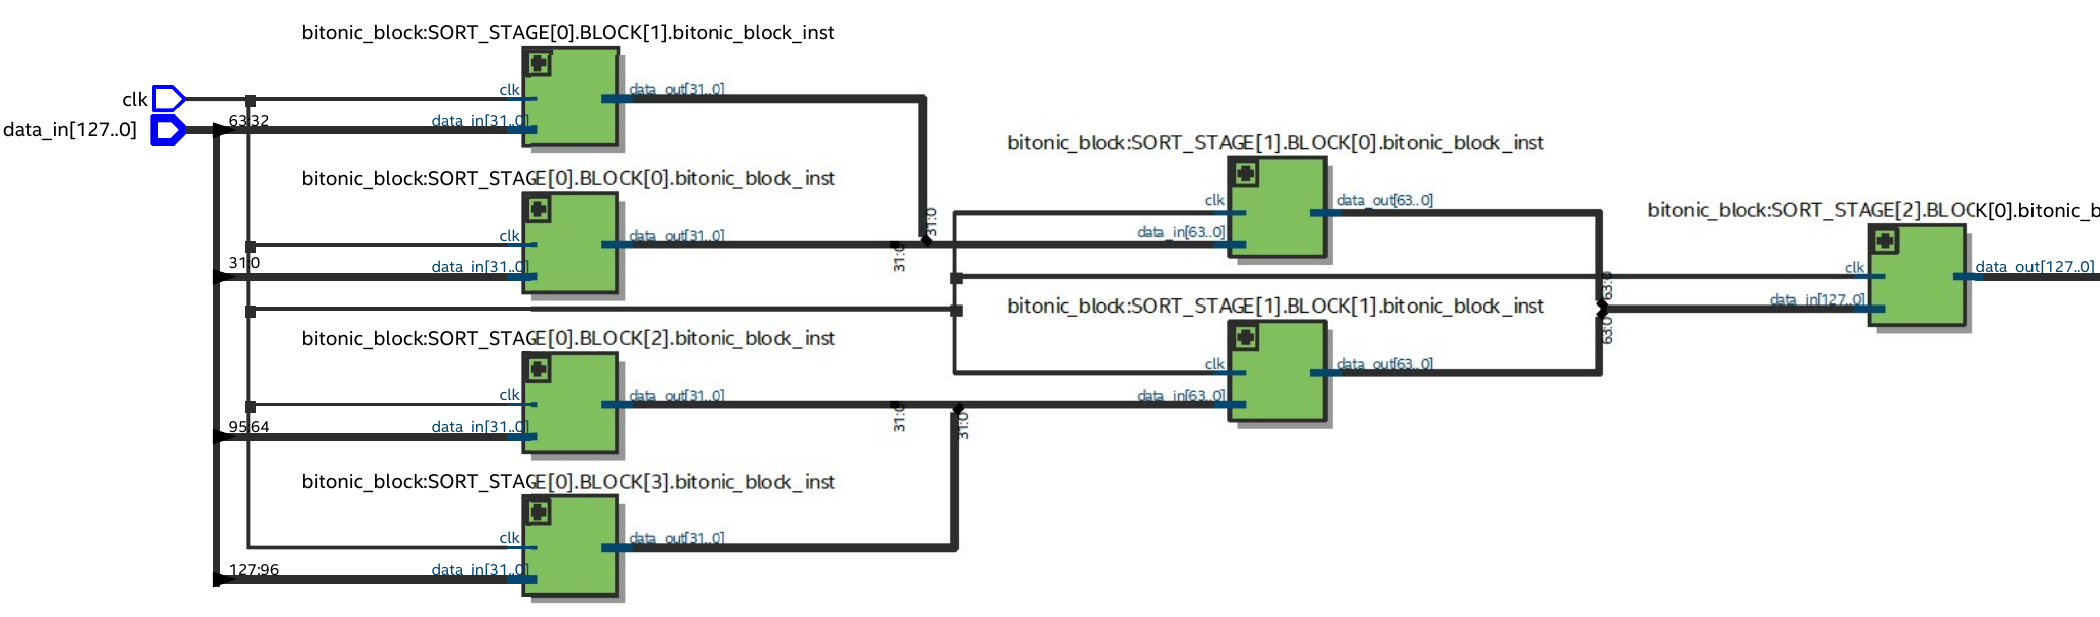
\includegraphics[scale=0.28]{slike/rtl_verilog2.png}
  \caption{Слика добијеног кола - RTL View}
  \label{fig:rtl_verilog}
\end{figure}

Слика \ref{fig:rtl_verilog} је добијена коришћењем RTL View унутар алата Quartus Prime Lite и представља сортер осам 16-битних бројева добијен овом имплементацијом у Верилогу. Може се приметити да се мрежа састоји из три нивоа. Број нивоа се рачуна унутар \verb+bitonic_sort+. У овом случају параметар \verb+CHAN_NUM+ износи 8 па је број нивоа у мрежи 3, у случају да је потребно сортирати 16 елемената број нивоа би био 4. Приказан је део програмског код модула \verb+bitonic_sort+. Број блокова у нивоу се дефинише у параметру \verb+BLOCKS+.

\begin{minted}[frame=single,framesep=6pt]{verilog}
localparam CHAN_ACT = 2**$clog2(CHAN_NUM);
localparam STAGES = $clog2(CHAN_ACT);
generate for (stage = 0; stage < STAGES; stage = stage + 1)
  begin: SORT_STAGE
	localparam BLOCKS = CHAN_ACT / 2**(stage+1);
	localparam BLOCK_ORDER = stage;

	wire [STAGE_DATA_WIDTH-1:0]stage_data_in;
	wire [STAGE_DATA_WIDTH-1:0]stage_data_out;
	assign stage_data_in = stage_data[stage];
	assign stage_data[stage + 1] = stage_data_out;
	for (block = 0; block < BLOCKS; block = block + 1) begin: BLOCK
\end{minted}

Модул \verb+bitonic_block+ (из првог нивоа) је приказан на слици \ref{fig:rtl_verilogSub}. Следеће линије програмског код део су \verb+bitonic_block+ модула, параметар је \verb+ORDER+ једнак трунутном нивоу унутар мреже, па ће нпр.\ број инстанци \verb+bitonic_node+-а које су део \verb+bitonic_block+-а другом нивоу мреже бити $2^0 + 2^1 = 3$ (постоје два нивоа унутар блока).

\begin{minted}[frame=single,framesep=6pt]{verilog}
 localparam STAGES = ORDER + 1;
 generate for (stage = 0; stage < STAGES; stage = stage + 1)
  begin: BLOCK_STAGE
	localparam NODES = 2**stage;
	localparam NODE_ORDER = STAGES - stage - 1;
\end{minted}

Број инстанци \verb+bitonic_comp+ унутар једног \verb+bitonic_node+-а је већи што је он ближи улазу, а тај број је дефинисан као 2 на степен колико је сам \verb+bitonic_node+ удаљен од излаза из блока, нпр.\ онај до излаза ће имати $2^0=1$ инстанцу.
\begin{figure}[H]
  \centering
      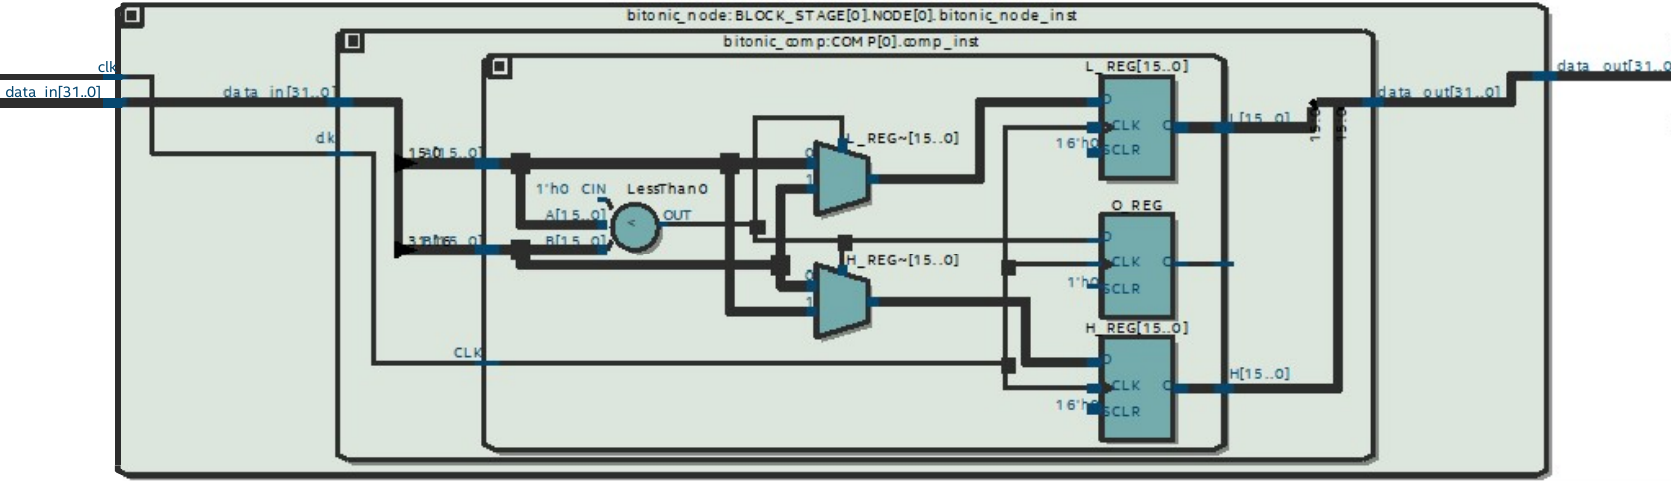
\includegraphics[scale=0.35]{slike/rtl_verilogSub2.png}
  \caption{Приказ подмодула у добијеном колу - RTL View}
  \label{fig:rtl_verilogSub}
\end{figure}


\subsubsection{Карактеристике генерисаног кола}
Синтеза и симулација рада битоник сортера је урађена у Quartus Prime Lite, а FPGA уређај коришћен за синтезу је Cyclone V 5CGXFC9E7F35C8.
\begin{table}[H]
\centering
 \begin{tabular}{| c | c | c c c |}
  \hline
  Број ел. & Ширина & LUT & Reg & Pin \\
  \hline
  8 & 8  & 325 & 455 & 129 \\
  8 & 16 & 620 & 867 & 257 \\
  8 & 32 & 1217 & 1602 & 513 \\
  \hline
  16 & 8 & 1100 & 1609 & 257 \\
  16 & 16 & 2067 & 2788 & 513 \\
  \hline
 \end{tabular}
 \caption{Простор који синтеза заузима за различите величине улаза}
 \label{tab:cipSinteza}
\end{table}
Табела \ref{tab:cipSinteza} приказује колико простора синтеза кода заузима простора на чипу, за различите величине улаза (и излаза). За различит број елемената на улазу и ширину података приказане су у колонама: LUT се односи на број искоришћених Look-Up табела, колона Reg представља укупан број потребних регистара, a Pin је искоришћен број пинова потребних за У/И.

Табела \ref{tab:sim} приказује број тактних циклуса потребних да се добије сортиран низ на излазу кола. Симулација је извршена за различите величину улаза (и излаза) и различите низове (насумични, скоро сортирани и обрнуто сортирани низови).

\begin{table}[H]
\centering
 \begin{tabular}{| c | c | c c c |}
  \hline
  Број ел. & Ширина & Насумични & Скоро с. & Обрнуто с. \\
  \hline
  8 & 8  & 6 & 6 & 6 \\
  8 & 16 & 6 & 6 & 6 \\
  8 & 32 & 6 & 6 & 6 \\
  \hline
  16 & 8 & 10 & 10 & 10 \\
  16 & 16 & 10 & 10 & 10 \\
  \hline
 \end{tabular}
 \caption{Број тактних циклуса за различитe низове и величину улаза}
 \label{tab:sim}
\end{table}

Следећа слика приказује симулацију улазног низа од 16 бројева коришћењем EDA алата Questa у оквиру Quartus Prime Lite.

\begin{figure}[H]
  \centering
      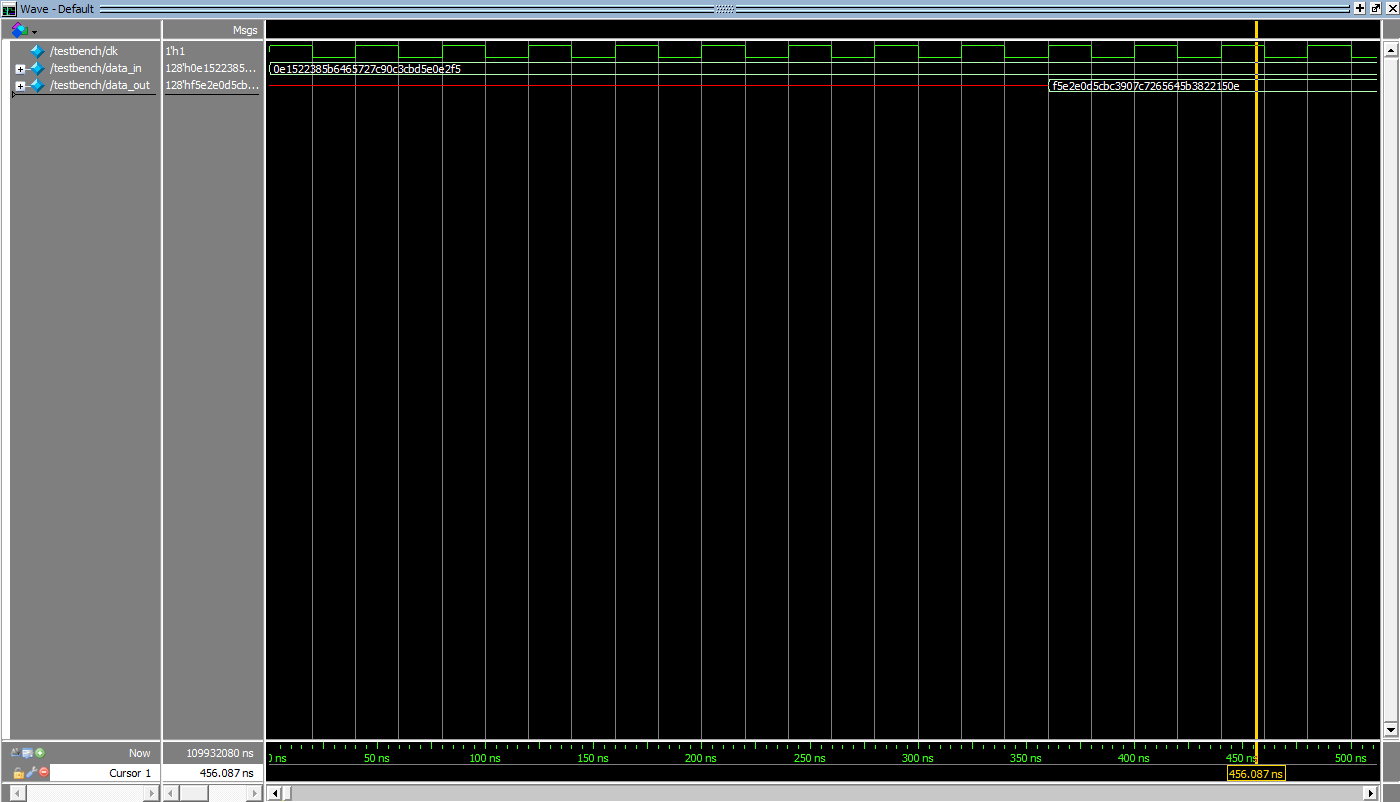
\includegraphics[scale=0.4]{slike/quartusSim.png}
  \caption{Симулација добијеног кола за сортирање 16 елемената}
  \label{fig:quartusSim}
\end{figure}

\newpage
\subsection{Имплементација битоник сортера у Верилогу - комбинациона}
Сада ће бити описана једноставна имплементација битоник сортера у Верилогу \cite{git_verilogProsto}, коло које се добије је секвенцијално, а број елемената који се сортирају је \mbox{фиксан (16)} и ширина података је 16. Сада ће бити описан програмски код:
\begin{enumerate}
 \item Модул \verb+BN+ има два 16-битна улаза \verb+a+ и \verb+b+ и два 16-битна излаза, \verb+min+ и \verb+max+. Излазне вредности се дефинишу као:
 \begin{minted}[frame=single,framesep=6pt]{verilog}
assign min = (a < b) ? a : b;
assign max = (a < b) ? b : a;
 \end{minted}
  \item Модул \verb+BN1+ је сличан \verb+BN+, али мења редослед излаза; прво \verb+max+, па \verb+min+.
\item Модул \verb+sorting+ је главни модул за сортирање који сортира 8 16-битних вредности. Улази су \verb+a1+ до \verb+a8+, излази \verb+b1+ до \verb+b8+. Може се рећи да је ова имплементација „хардкодована” репрезентација битоник мреже за сортирање као на сликама \ref{fig:bitonicStages} или \ref{fig:RTL_Iter}. Сваки ниво мреже се експлицитно дефинише и спаја жицама. Иако једноставно решење, није параметризовано и може се користити само за фиксан број елемената на улазу.
\begin{minted}[frame=single,framesep=6pt]{verilog}
BN m21(a1,a2,mnn1,mxx1);
BN1 m22(a3,a4,mnn2,mxx2);
BN m23(a5,a6,mnn3,mxx3);
BN1 m24(a7,a8,mnn4,mxx4);
 \end{minted}
\end{enumerate}
\subsubsection{Карактеристике добијеног кола}
Извршена је синтеза и симулација овог кола. Следећа табела описује простор који генерисано коло заузима на чипу.

\begin{table}[H]
\centering
 \begin{tabular}{| c | c | c c |}
  \hline
  Број ел. & Ширина & LUT & Pin \\
  \hline
  16 & 8  & 929 & 256 \\
  16 & 16 & 2154 & 512 \\
  \hline
 \end{tabular}
 \caption{Простор који синтеза заузима за различите величине улаза}
 \label{tab:cipSintezaVer1}
\end{table}

На слици добијеној коришћењем RTL view из алата Quartus, може се приметити да се заправо ради о истом решењу као што је претходно описана итеративна у Чизелу (осим што \verb+BN+ и \verb+BN1+ имају окренуте излазе).

\newpage
\section{Рекурзивна имплементација битоник сортера у Чизелу - резултат рада}

 Две имплементације описане у претходном поглављу су коришћене као основа за израду ове, где је прва коришћена као референца за синтаксу Чизела, а друга као логичка основа. Оно што је било изазовно је размевање начина рада итеративне имплементације где се прави посебна инстанца модула за замену два елемента \verb+Swapper+ и излаз додељује новом низу, који је повратна вредност функцкије \verb+insertSorter()+. То значи да приступ примењен у рекурзивној Пајтон имплементацији није могућ а да коло истовремено буде секвенцијално, јер се ту мења улазни низ. Потребно је било написати рекурзивну имплементацију у Чизелу где функције \verb+sort+, \verb+bitonicSort+ и \verb+bitonicMerge+ као повратну вредност имају низ тј.\ \verb+IndexedSeq[Option[T]]+, а рекурзивним позивима функција се прослеђују само делови улазног низа.

Да би се генерисала нова листа са замењеним (свапованим) елементима у одговарајућем редоследу, у \verb+bitonicMerge()+ функцији, искорићена је \verb+foldLeft()+ функција, која извршава функцију \verb+swapIfNecessary()+.
Потом се долази до проблема саме замене елемената и на овом примеру се може видети како су Скала и Чизел сједињени и зашто је бити јасно разграничити типове података.
% Наиме, функција \verb+swapIfNecessary()+ мора имати повратну вредност и не може се враћати унутар Чизел \verb+when+ блока, а потребно је користити \verb+when+ зато што вршимо замену на основу Чизел \verb+Bool+ вредности, и њему дефинисати вредност неког сигнала, притом Скала \verb+if+ услов се може само користи уз Скала \verb+Boolean+.

% \begin{minted}[frame=single,framesep=6pt]{scala}
% val m = Module(new Passthrough(si.cloneType))
% val swapNeeded = lt(sj, si) === ascending
% when(swapNeeded) {
%   m.io.a0 := sj
%   m.io.a1 := si
% }.otherwise {
%   m.io.a0 := si
%   m.io.a1 := sj
% }
% seq.updated(i, Some(m.io.z0)).updated(j, Some(m.io.z1))
% \end{minted}

На крају, прави се инстанца једноставног модула \verb+Passthrough+ који само прослеђује вредности са улаза, и излаз се додељује новој листи, а на улазу се у зависности од \verb+swapNeeded+ елементи прослеђују у обрнутом или истом редоследу. Ако би се слично као у итеративној имплементацији прослеђивала \verb+Bool+ вредност \verb+swapNeeded+ модулу \verb+Swapper+, Чизел би пријавио грешку да не види ову вредност из модула \verb+Swapper+, па је на овај начин решен тај проблем.

\subsection{Опис програма}

Сада ће бити описан програмски код имплементације изложене у овом раду:
\begin{enumerate}
\item \verb+Passthrough+ је једноставан модул који има два улазна порта \verb+a0+ и \verb+a1+ и два излазна порта \verb+z0+ и \verb+z1+. Прихвата два податка истог типа \verb+T+ и директно их рутира на излазне портове без измене.

\item Објекат \verb+BitonicSorter+ дефинише функције за имплементацију битоник сорт алгоритма: \verb+bitonicMerge()+, \verb+bitonicSort()+ и \verb+sort()+.

\item Функција \verb+bitonicMerge()+ прима низ елемената \verb+arr+, дужину низа \verb+length+, информацију о редоследу сортирања \verb+ascending+, и функцију за упоређивање два елемента \verb+lt()+.
\begin{itemize}
\item Унутрашња функција \verb+swapIfNecessary()+ прихвата низ типа \verb+IndexedSeq[Option[T]]+, целобројни параметар \verb+i+, логичку вредност \verb+ascending+ и функцију за поређење \verb+lt()+ као параметре.
Ова функција је одговорна за замену два елемента у улазном низу ако је то потребно на основу функције поређења и флега ascending. Елементи се замењују кроз модул \verb+Passthrough+ и то зато што је било потребно користити услов \verb+when+ јер се проверава вредност \verb+swapNeeded+ која је типа \verb+Chisel.Bool+.
\newpage
На улазе овог модула се прослеђују вредности које су замењене или не, а излази \verb+m.io.a0+ и \verb+m.io.a1+ се уписују излазној секвенци.
\begin{minted}[frame=single,framesep=6pt]{scala}
def swapIfNecessary(seq: IndexedSeq[Option[T]], i: Int,
 ascending: Bool, lt: (T, T) => Bool):IndexedSeq[Option[T]]={
  val j = i + length / 2
  val si = arr(i).getOrElse(0.U.asTypeOf(arr(i).get))
  val sj = arr(j).getOrElse(0.U.asTypeOf(arr(j).get))
  val m = Module(new Passthrough(si.cloneType))
  val swapNeeded = lt(sj, si) === ascending
  when(swapNeeded) {
    m.io.a0 := sj
    m.io.a1 := si
  }.otherwise {
    m.io.a0 := si
    m.io.a1 := sj
  }
  seq.updated(i, Some(m.io.z0)).updated(j, Some(m.io.z1))
}
\end{minted}
\item Ако је дужина низа \verb+arr+ 1 или мања, низ се сматра већ сортираним и враћа се без промена.
\item Ако је дужина низа већа од 1, низ се дели на две половине и за сваки пар елемената \verb-(i, i+length/2)- се врши позив функције \verb+swapIfNecessary()+ над овим индексима коришћењем \verb+foldLeft()+.
\begin{minted}[frame=single,framesep=6pt]{scala}
val swappedSeq = indices.foldLeft(arr) { (seq, i) =>
  swapIfNecessary(seq, i, ascending, lt) }
\end{minted}
\item Након што се обаве сви кораци, сортиран низ се враћа као излаз функције.
\end{itemize}
\item Функција \verb+bitonicSort()+ прима низ елемената \verb+arr+ који треба сортирати, информацију о редоследу сортирања \verb+ascending+ - да ли је сортирање у растућем редоследу или не, и функцију за упоређивање два елемента \verb+lt+.
\begin{itemize}
 \item Ако је дужина низа \verb+arr+ 1 или мања, низ се сматра већ сортираним и враћа се без промена
 \item Ако је дужина низа већа од 1, врше се рекурзивни позиви половина низа у растућем и опадајућем редпоследу; а потом се две половине спајају користећи \verb+bitonicMerge()+.
 \item Након што се обаве сви кораци, сортиран низ се враћа као излаз функције.
\end{itemize}
\begin{minted}[frame=single,framesep=6pt]{scala}
def bitonicSort[T<:Data](arr: IndexedSeq[Option[T]], ascending: Bool,
                      lt: (T, T) => Bool): IndexedSeq[Option[T]] = {
  val n = arr.length
  if (n > 1) {
    val half = n / 2
    val left = bitonicSort(arr.slice(0, half), true.B, lt)
    val right = bitonicSort(arr.slice(half, n), false.B, lt)
    val merged = bitonicMerge(left ++ right, n, ascending, lt)
    merged
  } else {
    arr } }
\end{minted}
\item Функција \verb+sort()+ проверава да ли је дужина улазног низа 1 и ако јесте враћа га као излазну вредност, а ако је већа од 1 позива функцију \verb+bitonicSort()+ за извршење сортирања.
\item  Класа \verb+SorterModuleIfc+ дефинише интерфејс за модул битоник сортера. Као параметре прима број елемената за сортирање \verb+n+ и тип податка елемената \verb+proto+. Овде су дефинисани улаз \verb+a+ и излаз \verb+z+.
\item Класа \verb+BitonicSorterModule+ представља стварни модул битоник сортера који би се користио у хардверском дизајну.
\begin{itemize}
 \item Kао улазне параметре прихвата број елемената за сортирање \verb+n+, тип податка елемената \verb+proto+, флeг за редослед сортирања \verb+ascending+ и функцију за упоређивање \verb+lt+.
 \item Проверава се да ли је улзани низ степен броја 2 и избацује изузетак ако није испуњен овај услов.
 \item Креира интерну секвенцу \verb+a+ која се користи за сортирање. Елементи ове секвенце се изводе из улазних података \verb+io.a+, обезбеђујући да дужина секвенце буде степен броја \verb+2+.
 \begin{minted}[frame=single,framesep=6pt]{scala}
IndexedSeq.tabulate(if (n <= 1) 1 else 1<<log2Up(io.a.length)) {
  i => if (i < n) Some(io.a(i)) else None }
\end{minted}
 \item Сортиран излаз се израчунава помоћу функције \verb+BitonicSorter.sort()+ и додељује се излазном порту \verb+io.z.+
\end{itemize}

\item Примери генерисања кода \verb+BitonicSorterUInt8_64Driver+ и \verb+BitonicSorterUInt8_384Driver+ демонстрирају како користити модул битоник сортера са конкретним конфигурацијама, тако што се креирају инстанце \verb+BitonicSorterModule+ са различитим параметрима (нпр.\ сортирају 64 елемента типа \verb+UInt(8)+ у растућем редоследу) и генеришу SystemVerilog код користећи \verb+ChiselStage+.

\end{enumerate}

\newpage
\subsection{Тест за битоник сортер}
Сада ће бити описано тестирање рекурзивне имплементације битоник сортера, где се користе библиотеке \verb+ChiselTest+ и \verb+ScalaTest+.
\begin{enumerate}
 \item Класа \verb+BitonicSorterModuleTest+ је главна тест класа која проширује \verb+AnyFlatSpec+ из \verb+ScalaTest+ и \verb+ChiselScalatestTester+. Користи се за тестирање \verb+BitonicSorterModule+-a.
 \begin{minted}[frame=single,framesep=6pt]{scala}
class BitonicSorterModuleTest extends AnyFlatSpec
                                  with ChiselScalatestTester {
def generateRandomInput(size: Int, len: Int): Seq[UInt] = {
  Seq.fill(len)(BigInt(size, Random).U(size.W))
}
 \end{minted}
 \item Функција \verb+generateRandomInput+ генерише случајни низ улазних вредности \verb+UInt+. Прима два параметра: \verb+size+ (број битова сваког елемента) и \verb+len+ (број елемената у низу). Користи \verb+Seq.fill()+ да креира низ случајних \verb+UInt+ вредности са наведеним величинама.
 \begin{minted}[frame=single,framesep=6pt]{scala}
val lengths = Seq(1, 2, 4, 8, 16)
val randomIndex = Random.nextInt(lengths.length)
val length = lengths(randomIndex)
test(new BitonicSorterModule(length, UInt(bitSize.W), false.B,
                            (x: UInt, y: UInt) => x < y)) { dut =>
  val input = generateRandomInput(bitSize, length)
  dut.io.a.zipWithIndex.foreach { case (inputPort, index) =>
    inputPort.poke(input(index))}
 \end{minted}

 \item Тестни случајеви:
 \begin{itemize}
  \item Први тест случај проверава да ли \verb+BitonicSorterModule+ исправно сортира улазне вредности у растућем редоследу за различите величине података (8, 16, 32 и 64). Генерише случајне низове улазних вредности различитих дужина (1, 2, 4, 8 и 16) за сваку ширине података и проверава да ли излазне вредности одговарају растућем редоследу.
  \begin{minted}[frame=single,framesep=6pt]{scala}
// Check if the output values are in descending order
val veryLargeNumber = BigInt("922337203685477580755555")
var prevValue = veryLargeNumber
dut.io.z.foreach { outputPort: UInt =>
  val value = outputPort.peek().litValue //.toInt
  //println(value)
  outputPort.expect(value.U)
  assert(value <= prevValue,
            "Output values are not in descending order.")
  prevValue = value }
  \end{minted}

  \item Други тест случај је сличан првом, али проверава да ли модул исправно сортира улазне вредности у опадајућем редоследу. Такође тестира за различите ширине података и случајне дужине улаза.
  \begin{minted}[frame=single,framesep=6pt]{scala}
it should """not allow construction of Arrays whose length
        is not a power of 2""" in {
  assertThrows[IllegalArgumentException] {
          new BitonicSorterModule(7,
            UInt(8.W), true.B, (x: UInt, y: UInt) => x < y) }
  \end{minted}

  \item Трећи тест случај проверава да ли конструктор \verb+BitonicSorterModule+ баца \verb+IllegalArgumentException+ када се покуша креирање инстанце са дужином улаза која није степен броја 2.
 \end{itemize}
\end{enumerate}


\begin{figure}[H]
  \centering
      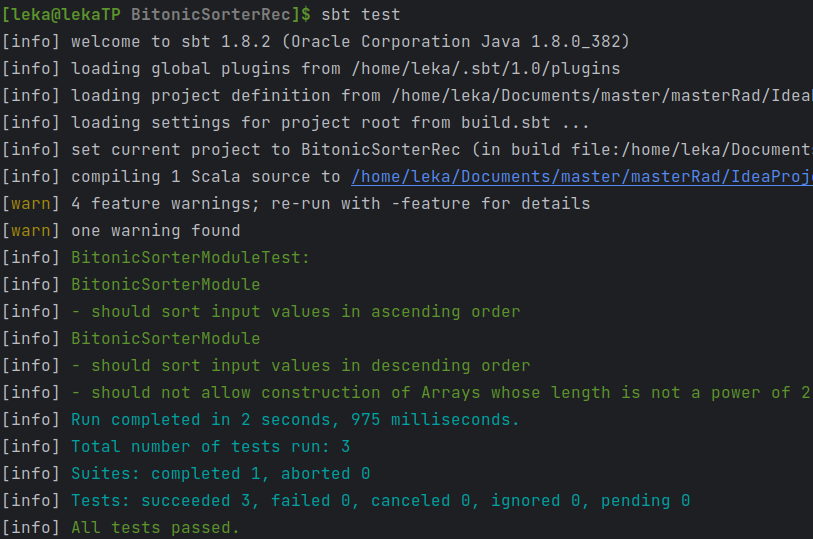
\includegraphics[scale=0.5]{slike/testRes2}
  \caption{Извршавање теста}
  \label{fig:testRes}
\end{figure}

\newpage
\subsection{Покретање програма}
У GitHub репозиториjуму \textit{BitonicSorterRecursive}, наведеном у литератури \cite{git_moje}, се налазе:
\begin{itemize}
\item Пројекат \textit{BitonicSorterRec}, који се може отворити у Intellij-у
\item \LaTeX{} код овог рада и pdf датотека
\end{itemize}

Покретање пројекта се врши извршавањем команде \verb+sbt test+ у директоријуму пројекта.

\begin{figure}[H]
  \centering
      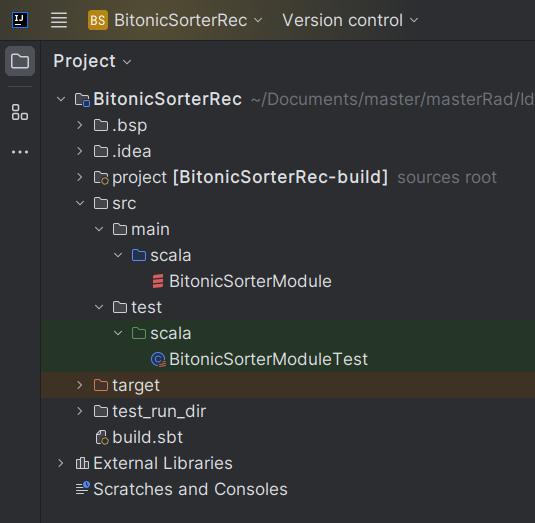
\includegraphics[scale=0.5]{slike/struktura}
  \caption{Структура пројекта}
  \label{fig:struktura}
\end{figure}

Слика \ref{fig:struktura} приказује структуру пројекта, \verb+BitonicSorterModule.scala+ се налази у директоријуму \verb+/src/main/scala/+, a \verb+BitonicSorterModuleTest.scala+ у \verb+/src/test/scala/+.
Слика \ref{fig:testRes} приказује резултат извршавања теста.

\newpage
\subsection{Приказ добијеног кола}

Слика \ref{fig:visualizeRec} прикатује генерисано коло овако имплементираног битоник сортера и на први поглед изгледа сложеније него коло имплементирано итеративним приступом.

\begin{figure}[H]
  \centering
      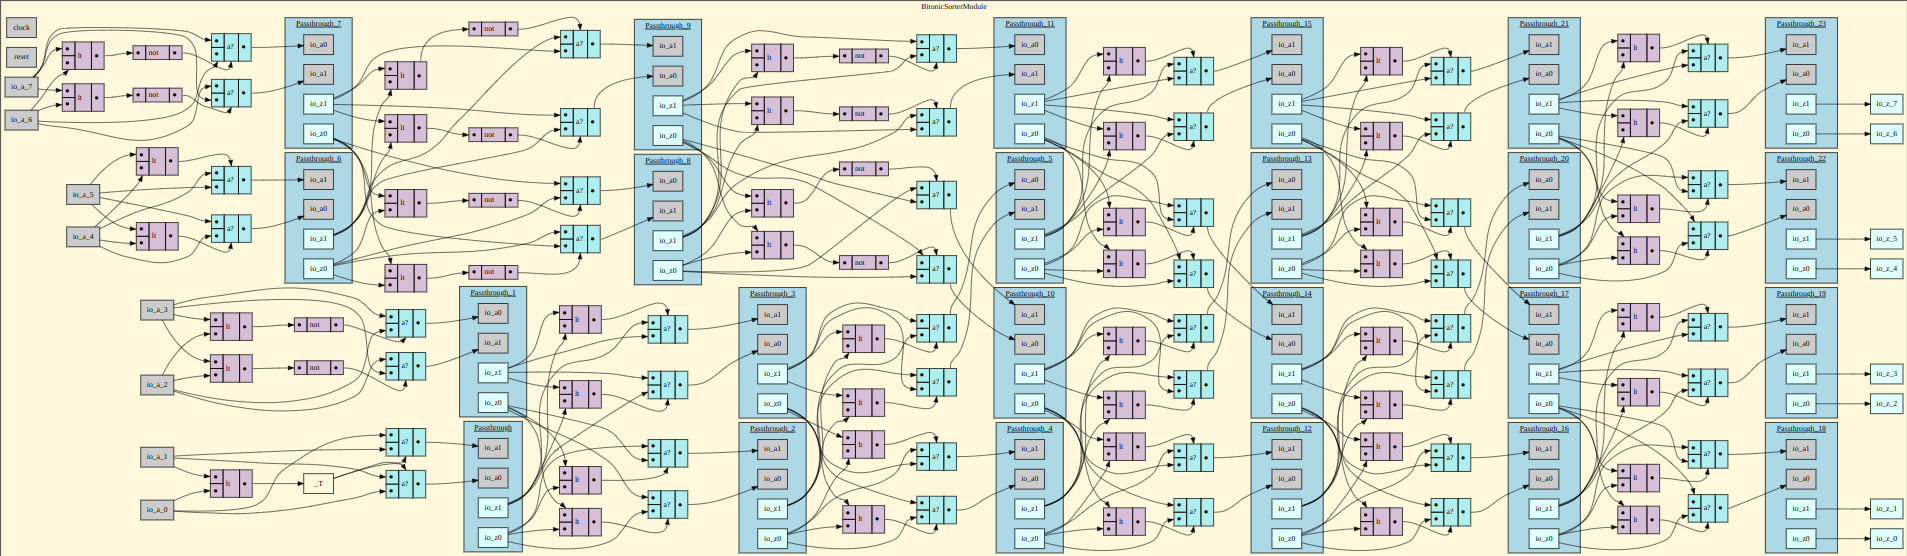
\includegraphics[scale=0.31]{slike/visualizeRec.png}
  \caption{Приказ рекурзивне имплементације}
  \label{fig:visualizeRec}
\end{figure}

Програмски код итеративне имплементације модул \verb+Swapper+ независно врши замену елемената, док су овде у замену укључени модул \verb+Passthrough+, функција поређења \verb+lt()+, \verb+ascending+ и може се видети негација \verb+not+; али су то су елементи који се понављају.

\subsection{Карактеристике генерисаног кола}
Позивом \verb+getVerilog(new BitonicSorterModule(...)+ је добијен Верилог програмски код рекурзивне имплементације. Синтеза и симулација рада битоник сортера је урађена у софтверу Quartus Prime Lite, резултати су приказани у наредној табели.
\begin{table}[H]
\centering
 \begin{tabular}{| c | c | c c |}
  \hline
  Број ел. & Ширина & LUT & Pin \\
  \hline
  8 & 8  & 347 & 130 \\
  8 & 16 & 676 & 258 \\
  8 & 32 & 1669 & 514 \\
  \hline
  16 & 8 & 931 & 258 \\
  16 & 16 & 2155 & 514 \\
  \hline
 \end{tabular}
 \caption{Простор који синтеза заузима за различите величине улаза}
 \label{tab:cipSintezaRec}
\end{table}
Може се приметити да су вредности у колонама LUT и Pin готово исте као у случају синтезе кола претходно описане итеративне имплементације у Чизелу.

Слика \ref{fig:RTL_Rec} приказује генерисано коло за сортирање 8 8-битних елемената, иако коло изгледа сложено, заправо се из табеле \ref{tab:cipSintezaRec} види заузумају исто простора на чипу.

\begin{figure}[H]
  \centering
      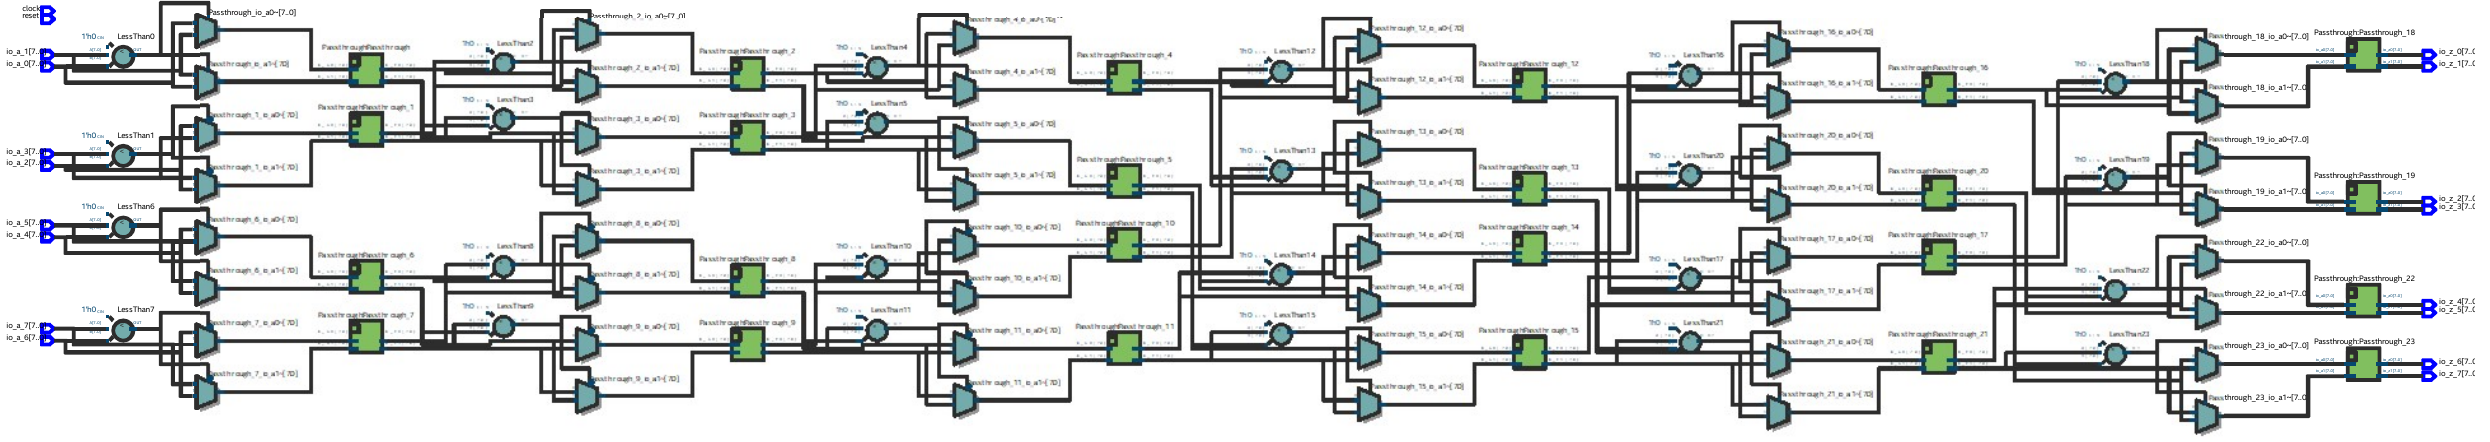
\includegraphics[scale=0.24]{slike/RTL_Rec_8_8.png}
  \caption{Слика добијеног кола за сортирање 8 елемената}
  \label{fig:RTL_Rec}
\end{figure}

\subsubsection{Поређење са претходним имплементацијама}
Следећи график приказује број Look-up табела потребних за синтезу приказаних имплементација на FPGA уређају Cyclone V 5CGXFC9E7F35C8 када је број елемената за сортирање 8.
\begin{figure}[H]
  \centering
      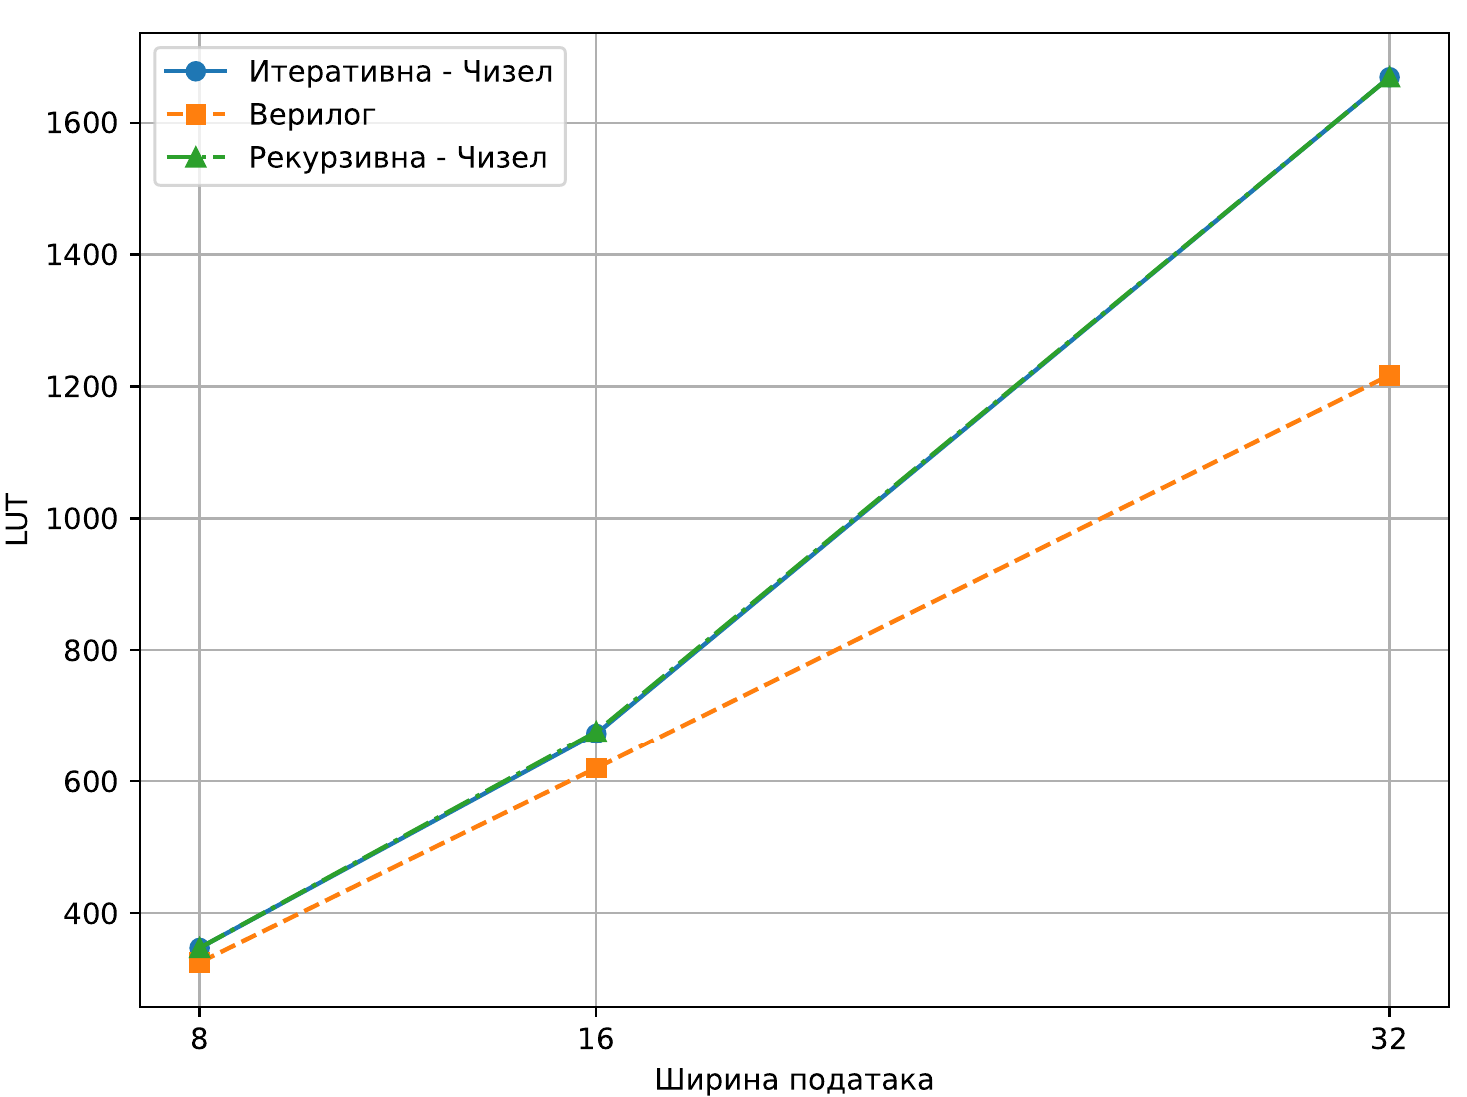
\includegraphics[scale=0.22]{slike/lut8}
  \caption{LUT - дужина низа 8}
  \label{fig:LUT8}
\end{figure}

График приказан на следећој слици приказује број Look-up табела када је дужина низа 16.
\begin{figure}[H]
  \centering
      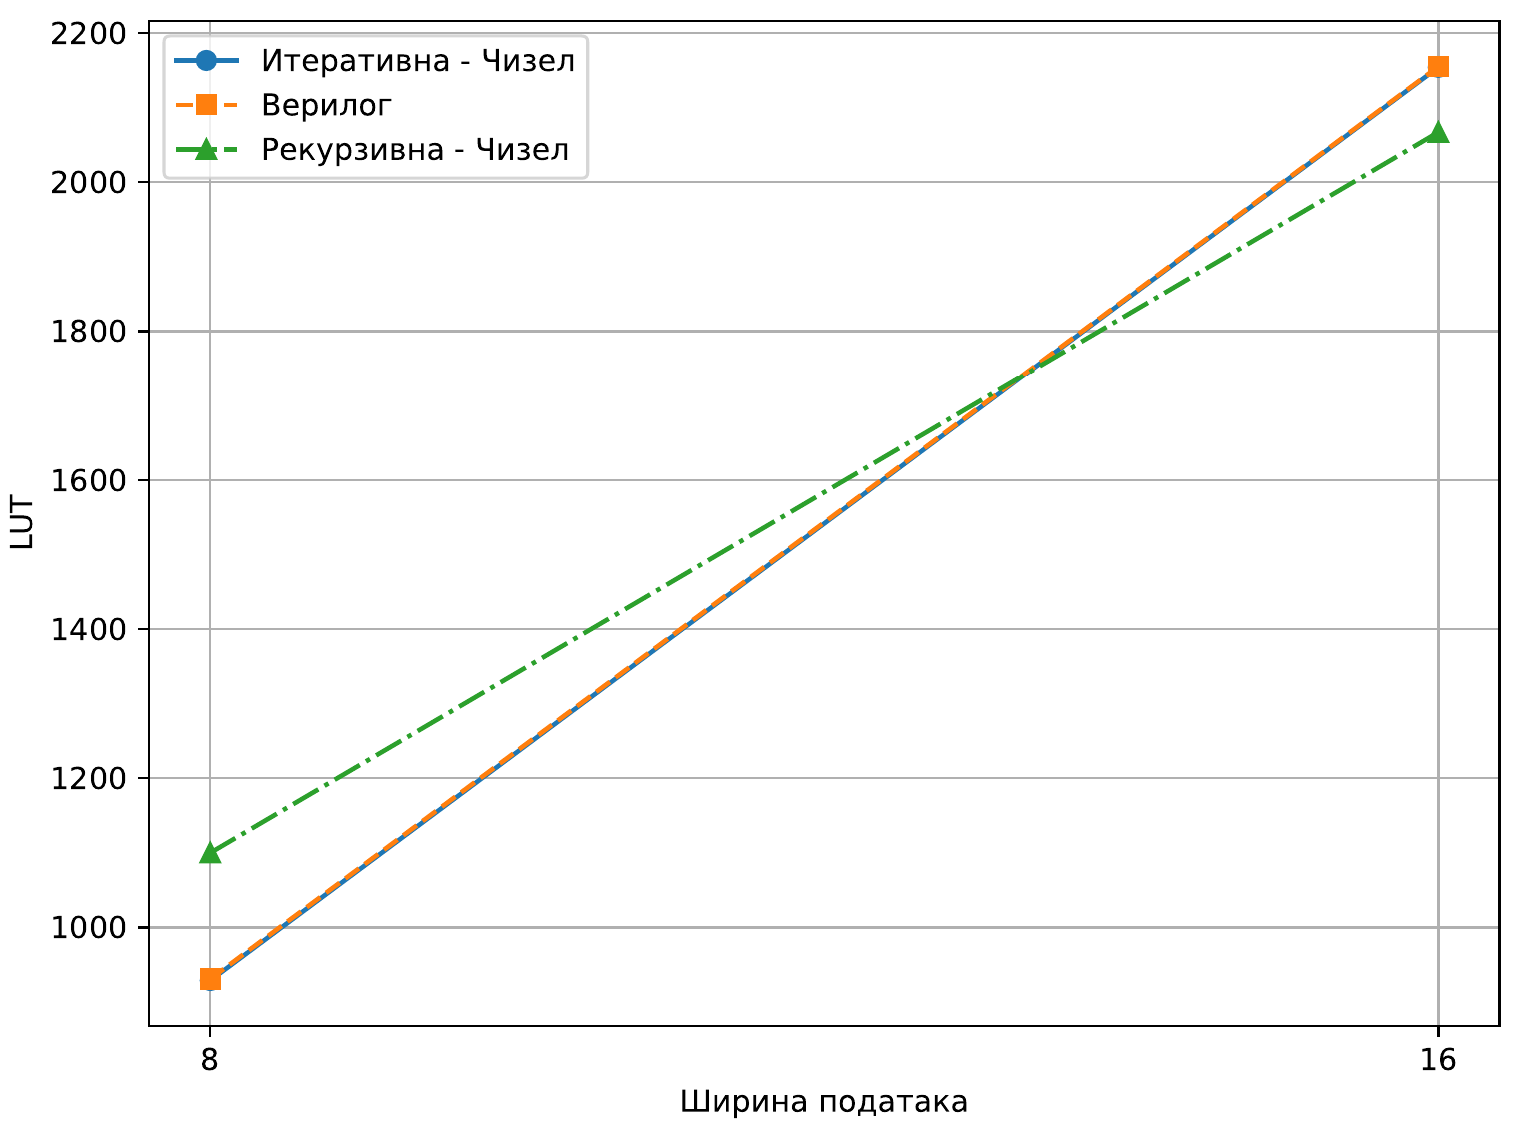
\includegraphics[scale=0.22]{slike/lut16}
  \caption{LUT - дужина низа 16}
  \label{fig:LUT16}
\end{figure}

Следећа табела приказује разлику у величини резултујућег Верилог кода ове имплементације у односу на приказано итеративно решење, зависно до величине улаза.

\begin{table}[H]
\centering
 \begin{tabular}{| c | c | c c |}
  \hline
  Број ел. & Ширина & Рекурзивна и. & Итеративна \\
  \hline
  8 & 8  & 356 & 327 \\
  8 & 16 & 368 & 327 \\
  8 & 32 & 368 & 327 \\
  \hline
  16 & 8 & 1158 & 1023 \\
  16 & 16 & 1158 & 1023 \\
  \hline
 \end{tabular}
 \caption{Простор који синтеза заузима за различите величине улаза}
 \label{tab:brojLinija}
\end{table}

Занимљиво је приметити да се у коду рекурзивне имплементације оператори примењују директно над жицама (\verb+wire+), и због тога се добије сложена шема кола после синтезе приказана на сликама \ref{fig:RTL_Rec} и \ref{fig:visualizeRec}.

\begin{minted}[frame=single,framesep=6pt]{verilog}
  wire  _T_2 = io_a_3 < io_a_2; // @[cmd4.sc 1:101]
  wire  _T_3 = ~_T_2; // @[cmd2.sc 36:35]
  wire  _T_4 = Passthrough_1_io_z0 < Passthrough_io_z0;
      // @[cmd4.sc 1:101]
  ...
  assign Passthrough_io_a0 = _T ? io_a_1 : io_a_0;
      // @[cmd2.sc 37:24 cmd2.sc 38:17 cmd2.sc 41:17]
  assign Passthrough_io_a1 = _T ? io_a_0 : io_a_1;
      // @[cmd2.sc 37:24 cmd2.sc 39:17 cmd2.sc 42:17]
  ...
  Passthrough Passthrough ( // @[cmd2.sc 35:21]
    .io_a0(Passthrough_io_a0),
    .io_a1(Passthrough_io_a1),
    .io_z0(Passthrough_io_z0),
    .io_z1(Passthrough_io_z1)
  );
\end{minted}

На основу ових исечака програмског кода може се закључити зашто резултује компликованом шемом кола.
\begin{table}[H]
\centering
 \begin{tabular}{| c | c | c c c |}
  \hline
  Број ел. & Ширина & Вер. & Рек. & Итер. \\
  \hline
  8 & 8  & 530.08 & 530.06 & 531.20 \\
  8 & 16 & 535.70 & 535.81 & 536.66 \\
  8 & 32 & 546.12 & 546.50 & 545.98 \\
  \hline
  16 & 8 & 535.41 & 535.40 & 535.59 \\
  16 & 16 & 546.31 & 545.60 & 546.36 \\
  \hline
 \end{tabular}
 \caption{Простор који синтеза заузима за различите величине улаза}
 \label{tab:potrosnja}
\end{table}
Tабела \ref{tab:potrosnja} приказује потрошњу енергије изражену у [mW], за рекурзивну, итеративну и имплементацију у Верилогу.

\newpage
\section{Закључак}

Чизел нуди могућност дизајнирања хардвера са начином размишљања као да је у питању програмирање у језику вишег нивоа. Самим тим програмирање је лакше, док се добија сличан код као да се директно програмира у језику за дизајн хардвера.

Током израде је било потребно разумети начин рада постојећих решења да би се превазишле разлике и ограничења у програмирању коришћењем програмских језика и језика за опис хардвера. Рекурзивна имплементација битоник сортера приказана у овом раду заузима исти простор на чипу као итеративна, иако шема на први поглед делује компликованије; а сам програмски код је интуитивнији. Код свих имплементација се може видети раст броја елемената у колу са порастом броја елемената за сортирање.


Добијена имплементација није преведена до фазе рутирања и временске анализе. У будућности може се анализирати на коликој фреквенцији ова имплементација може да ради, као и који делови се могу оптимизовати. Добијено коло изгледа сложено и шема би била прегледнија ако би имплементација била састављена од подмодула, а не појединачних оператора. Простор за унапређење би био да се додатно анализира битоник сорт алгоритам и уоче још неки начини рекурзивне имплементације чиме би се добила јаснија шема резултујућег кола.


%Несумњиво је да Чизел пружа могућност ефикаснијег куцања кода и једноставнијег описа хардвера.

%\newpage
\clearpage
\begingroup
\raggedright
%\bibliography{srpski_Literatura}


\begin{thebibliography}{99}

\bibitem{wiki_scala}
\textit{Scala (programming language)}, приступљено (август 2023.) на
\url{https://en.wikipedia.org/wiki/Scala_(programming_language)}

\bibitem{odersky2016}
  Martin Odersky, Lex Spoon, and Bill Venners,
  ``Programming in Scala, Third Edition'',
  Artima, 2016.

\bibitem{courseraHOF}
Martin Odersky, \textit{Higher-order functions}, [Интернет курс] \textit{Functional Programming Principles in Scala}, приступљено (август 2023.) на
\url{https://www.coursera.org/learn/scala-functional-programming/lecture/V5crF/lecture-2-1-higher-order-functions}

\bibitem{wiki_chisel}
\textit{Chisel (programming language)}, приступљено (август 2023.) на
\url{https://en.wikipedia.org/wiki/Chisel_(programming_language)}

% \bibitem{berkeley_twigg}
%   Stephen Twigg,
%   "Flexible FFT Optimization and RTL Generation in the Chisel Hardware Design Language" [Мастер рад, Универзитет у Калифорнији, Беркли],
%   Artima, 2016.

\bibitem{berkeley_twigg}
  Stephen Twigg,
  ``Flexible FFT Optimization and RTL Generation in the Chisel Hardware Design Language'', [Мастер рад, Универзитет у Калифорнији, Беркли], 2015.
  \url{http://www2.eecs.berkeley.edu/Pubs/TechRpts/2015/EECS-2015-256.html}

\bibitem{git_chisel}
\textit{Chisel Bootcamp}, приступљено (август 2023.) на
\url{https://github.com/freechipsproject/chisel-bootcamp.git}

\bibitem{zuluaga2016}
  Marcela Zuluaga, Peter Milder, and Markus Püschel,
  ``Streaming sorting networks'',
  ACM Trans.\ Des.\ Autom.\ Electron.\ Syst.\ 21, 4, чланак 55, 2016.
  \verb+DOI+:\url{http://dx.doi.org/10.1145/2854150}

\bibitem{bitonicBatcher}
  K.\ E.\ Batcher,
  ``Sorting networks and their applications'',
  ACM, 1968.
  \verb+DOI+:\url{http://dx.doi.org/10.1145/1468075.1468121}

\bibitem{wiki_bitonic}
\textit{Bitonic sorter}, приступљено (август 2023.) на
\url{https://en.wikipedia.org/wiki/Bitonic_sorter}

%%%%%%%%%%%%%%%%%%%%%%%%%%%%%%%%%%%%%%%%%%%%%%%%%%%%%%%%%%%%%
\bibitem{stone}
  H. S. Stone,
  ``Parallel processing with the perfect shuffle'',
  IEEE Transactions on Computers 20, 2, 153–161, 1971.
  \verb+DOI+:\url{http://dx.doi.org/10.1109/T-C.1971.223205}

\bibitem{preparata}
 Gianfranco Bilardi, Franco P. Preparata
  ``An architecture for bitonic sorting with optimal VLSI performance'',
  IEEE Transactions on Computers, 1984.
  \verb+DOI+:\url{http://dx.doi.org/10.1109/TC.1984.5009338}

\bibitem{dowd}
 Martin Dowd, Yehoshua Perl, Larry Rudolph, Michael Saks,
  ``The periodic balanced sorting network'',
  Journal of the ACM 36, 4, 738–757, 1989.
  \verb+DOI+:\url{http://dx.doi.org/10.1145/76359.76362}

\bibitem{layer04}
 Christophe Layer, Hans-Jörg Pfleiderer
  ``A reconfigurable recurrent bitonic sorting network for concurrently accessible data'',
   Field Programmable Logic and Application, 648–657, 2004.
  \verb+DOI+:\url{http://dx.doi.org/10.1007/978-3-540-30117-2_66}

\bibitem{layer07}
 Christophe Layer, Daniel Schaupp, Hans-Jörg Pfleiderer
  ``Area and throughput aware com-parator networks optimization for parallel data processing on FPGA'',
  Proceedings of the Interna-tional Symposium on Circuits and Systems, IEEE  405–408, 2007
  \verb+DOI+:\url{http://dx.doi.org/10.1109/ISCAS.2007.378475}

  \bibitem{zang}
 Y. Zhang, S. Q. Zheng
  ``An efficient parallel VLSI sorting architecture'',
  VLSI Design 11, 2, 137–147, 2000.
  \verb+DOI+:\url{http://dx.doi.org/10.1155/2000/14617}

  \bibitem{aitan}
  M. Ajtai, J. Komlós, and E. Szemerédi
  `` An O(N log N) sorting network.'',
  VLSI Design 11, 2, 137–147, 2000.
  \verb+DOI+:\url{http://dx.doi.org/10.1155/2000/14617}

  \bibitem{knuth}
  Donald E. Knuth,
  ``The Art of Computer Programming: Sorting and Searching'',
  Addison-Wesley, 1968.
%%%%%%%%%%%%%%%%%%%%%%%%%%%%%%%%%%%%%%%%%%%%%%%%%%%%%%%%%%%%

\bibitem{git_freeChipsBitonic}
Steve Burns,
\textit{Bitonic Sorter}, приступљено (септембар 2023.) на
\url{https://github.com/freechipsproject/ip-contributions/tree/master/src/main/scala/chisel/lib/bitonicsorter}

\bibitem{geeks}
\textit{Bitonic Sort}, приступљено (септембар 2023.) на
\url{https://www.geeksforgeeks.org/bitonic-sort/}

\bibitem{git_verilog}
\textit{Bitonic sorter - Verilog}, приступљено (септембар 2023.) на
\url{https://github.com/mcjtag/bitonic_sorter.git}

\bibitem{git_verilogProsto}
\textit{Bitonic sorter (Combinational) - Verilog}, приступљено (септембар 2023.) на
\url{https://digitalsystemdesign.in/bitonic-sorter/}

\bibitem{git_moje}
\textit{BitonicSorterRecursive}, приступљено (септембар 2023.) на
\url{https://github.com/aleksavelickovic5762015/BitonicSorterRecursive.git}

\end{thebibliography}

\endgroup

\newpage

\section*{Списак скраћеница}
\addcontentsline{toc}{section}{Списак скраћеница}
\begin{acronym}
\acro{fvr}[ФВР]{Функције вишег реда}
\end{acronym}

\listoftables

\newpage

\listoffigures


\end{document}
